\documentclass[conference]{IEEEtran}
\IEEEoverridecommandlockouts
% The preceding line is only needed to identify funding in the first footnote. If that is unneeded, please comment it out.
\usepackage[numbers]{natbib}
\usepackage{amsmath,amssymb,amsfonts}
\usepackage{algorithmic}
\usepackage{graphicx}
\usepackage{textcomp}
\usepackage{xcolor}
\def\BibTeX{{\rm B\kern-.05em{\sc i\kern-.025em b}\kern-.08em
    T\kern-.1667em\lower.7ex\hbox{E}\kern-.125emX}}

\begin{document}
\title{Smart concentrated liquidity}

\author{\IEEEauthorblockN{Stefan Duprey}
\IEEEauthorblockA{\textit{SwissBorg} \\
stefan@swissborg.com}
}

\maketitle

\begin{abstract}
Uniswap is the largest decentralized exchange (DEX) and one of cornerstones of Decentralized Finance (DeFi). Uniswap uses liquidity pools to provide Automated Market Making (AMM) functionality. Uniswap can provide more liquidity than its larger, centralized rivals Coinbase and Binance, because of the incentives it gives its liquidity providers to deliver better pricing to traders.\\
Uniswap version 3 is pioneering the new concept of concentrated liquidity feature, which allows the liquidity providers to concentrate their liquidity in a specific price range, leading to an increased capital efficiency compared to the previous v2 version.\\
However, the mathematical relationship between the liquidity position, the amount of assets in that position, and its price range becomes somewhat complex and the corollary to that capital efficiency is an even nastier impermanent loss risk than v2 when the initial price diverges from the initial entry price for the liquidity provision.\\
The ability to concentrate liquidity on uniswap V3 has been designed for people to gain efficiency on the capital they bring, but the key issue there is to find a suitable algorithm to rebalance the liquidity position bounds to maximize volume fees while keeping impermanent loss and rebalancing costs (transaction costs + swapping slippage) low.\\
One has to understand that the provision of liquidity in hyperbolic dexes will loose as soon as the price diverges (upwards or downwards) from where the initial price was when the liquidity was brought.\\
So liquidity provisioning has to be actively monitored. The chosen bounds must be actively managed to encompass the price moves and not get traversed.\\
In a volatile market, finding the right bounds for an optimal trading liquidity concentration is a challenging exercise : one has to find the optimal bounds rebalancing strategy for the perfect trade-off between impermanent loss, swapping costs and swapping volume fees generation.\\
Bullish/bearish market must be avoided at all costs : the market will traverse your bounds and leave you with your liquidity either in full stable coins in a bullish market or in full risky asset in a bearish market.\\
Passive liquidity investing must be seen as, in essence, a mean reverting strategy where the money is made from price fluctuation inside a specified range.\\
An algorithmic detection is therefore a must : one should discriminate markets as rangy, bullish or bearish and apply only passive liquidity provisioning in rangy markets.\\
We here detail the trade-off optimization problem to detect liquidity bounds algorithmically.
\\
\begin{description}
  \item[$\bullet$]Maximize price inside the tightest bounds to earn volume fees (the tighter the bounds, the efficienter the capital)
  \item[$\bullet$] Impermanent loss and swapping slippage costs incurred at each rebalancing have to be minimized
\end{description}
We here give a rebalancing methodology and the optimal matching parameters found by an exhaustive computational backtesting approach.\\
A proper analysis of the rebalancing costs versus fees generation is done.\\
An absolute performance analysis proves that the LP value fluctuation can be very corrosive when the underlying risky drops in value as both impermanent loss and 50\% risky position asset depreciation cumulate.\\
We then propose a new algorithm based on a trend detection signal where the loss in bearish market are mitigating by\\
\begin{description}
  \item[$\bullet$] Either shorting by using Aave money market
  \item[$\bullet$] Or hedging the LP position by buying an option basket for a specific maturity
  \item[$\bullet$] Or just shorting a perpetual according the delta of the LP position value (its sensitivity to the underlying)
\end{description}
\end{abstract}
\section{Understanding the risk of hyperbolic dexes (decentralized exchanges)}
\subsection{Hyperbolic equation}
Let $X$ denote the reserve of the risky asset (Ether, WBtc, SOL) and $Y$
denote the reserve of the non risky stable coin (USDT, USDC, BUSD, ..).
Uniswap pioneering approach was to force the reserve quantities on the pool to live on an hyperbole, hence the denomination hyperbolic dex.
\begin{equation}
    X * Y = cte = X_{t0} * Y_{t0}
\end{equation}
The constant is fixed by the initially brought amount at instant $t0$.
The risky asset price $X$ in stable coins $Y$ is directly linked to the pool reserve:
\begin{equation}
    P_{X \text{ in }Y}  = \frac{Y}{X} = P_X
\end{equation}
Basically if you have one Ether (X = 1) and 4500 USDT in the pool (Y = 4500), the ether
price is $\frac{4500}{1}$. And vice versa
\begin{equation}
    P_{Y \text{ in }X}  = \frac{X}{Y} = P_Y
\end{equation}
By denoting $L^2 = X_{t0} * Y_{t0}$ (L can be seen as the part of the liquidity brought by a single asset of the pool), a quick computation gives:
\begin{equation}
    L=\sqrt{X*Y}
\end{equation}
\begin{equation}
    X = \frac{L}{\sqrt{P_X}}  
\end{equation}
\begin{equation}
    Y = L*\sqrt{P_X}
\end{equation}

\subsection{Uniswap V2 Impermanent loss}
Uniswap V2 liquidity pools  are actively managed by arbitraging bots/traders which swap
the proper quantities to readjust the pool quantities to match the consensus price formed over all exchanges (centralized and decentralized).\\
Let's denote $t_1$ an instant where the pool quantities are denoted $X_{t_1}$, $Y_{t_1}$, $P_{X,t_1}$, $P_{Y,t_1}$.
Let's denote $t_2 > t_1$ a subsequent instant where the pool quantities are denoted $X_{t_2}$, $Y_{t_2}$, $P_{X,t_2}$, $P_{Y,t_2}$.

Let's imagine two different states of the reality. A first one where the pool has not been arbitraged and a second one where the pool has been arbitraged.

The quantities at instant $t_2$ when the pool has been arbitraged match the consensus price $P_{consensus}$:
\begin{equation}
    P_{X_{t_2}} = \frac{Y_{t_2}}{X_{t_2}} = P_{consensus}
\end{equation}

If the pool has not been arbitraged, its reserve quantities have not moved : they stayed at $X_{t_1}$, $Y_{t_1}$, $P_{X,t_1}$, $P_{Y,t_1}$.
\begin{equation}
    P_{X_{t_1}} = \frac{Y_{t_1}}{X_{t_1}}  \neq P_{consensus}
\end{equation}

Both state values of the pool in stable coins Y can be expressed as :
\begin{equation}
    V_{t_1} = X_{t_1}*P_{consensus} + Y_{t_1} = X_{t_1}*P_{X_{t_2}} + Y_{t_1}
\end{equation}
\begin{equation}
    V_{t_2} = X_{t_2}*P_{consensus} + Y_{t_2} = X_{t_2}*P_{X_{t_2}} + Y_{t_2}
\end{equation}
A quick computation gives the impermanent loss formula (the risk of loss for a non
arbitraged pool whose risky asset price has moved :
\begin{equation}
    \frac{v_{t_2} - v_{t_1}}{v_{t_1}} = \frac{2*\sqrt{\frac{P_{X_{t_2}}}{P_{X_{t_1}}}}}{1+\frac{P_{X_{t_2}}}{P_{X_{t_1}}}}-1
    =\frac{2*\sqrt{P_{X_{t_1}}P_{X_{t_2}}} - (P_{X_{t_1}} + P_{X_{t_2}}) } {P_{X_{t_1}} + P_{X_{t_2}}}
\end{equation}
This function is symmetrical in $P_{X_1}$ the price of the non-arbitraged pool at instant $t1$ and $P_{consensus} = P_{X_2}$ the consensus price at $t2$.
\\
The proof is straightforward :
$$
    \frac{v_{t_2} - v_{t_1}}{v_{t_1}} =     \frac{\frac{v_{t_2} - v_{t_1}}{X_{t_1}}} {\frac{v_{t_1}}{X_{t_1}}} = \frac{\frac{v_{t_2}}{X_{t_1}} - (P_{X_{t_1}} + P_{X_{t_2}})} {P_{X_{t_1}} + P_{X_{t_2}}}
$$
because $\frac{v_{t_1}}{X_{t_1}} = P_{X_{t_1}} + P_{X_{t_2}$.
$$
\frac{v_{t_2}}{X_{t_1}} =\frac{X_{t_2}*P_{X_{t_2}} + Y_{t_2}}{X_{t_1}} 
$$
$$
\frac{v_{t_2}}{X_{t_1}} ==\frac{2*Y_{t_2}}{X_{t_1}} =\frac{2*L*\sqrt{P_X_{t_2}}}{X_{t_1}}
$$
$$
\frac{v_{t_2}}{X_{t_1}} =\frac{2*L*\sqrt{P_X_{t_1}P_X_{t_2}}}{P_X_{t_1} * X_{t_1}} 
$$
$$
\frac{v_{t_2}}{X_{t_1}} =\frac{2*L*\sqrt{P_X_{t_1}P_X_{t_2}}}{\sqrt{P_X_{t_1}} * X_{t_1}} = 2* \sqrt{P_X_{t_1}P_X_{t_2}}
$$

By renaming $\frac{P_{X_{t_2}}}{P_{X_{t_1}}} = \tau $
We can rewrite the impermanent loss equation :
\begin{equation}
    \frac{v_{t_2} - v_{t_1}}{v_{t_1}} = \frac{2*\sqrt{\tau}}{1+\tau}}-1 = IL_{v2}(\tau)
\end{equation}
\begin{figure}[h!]
    \centering
    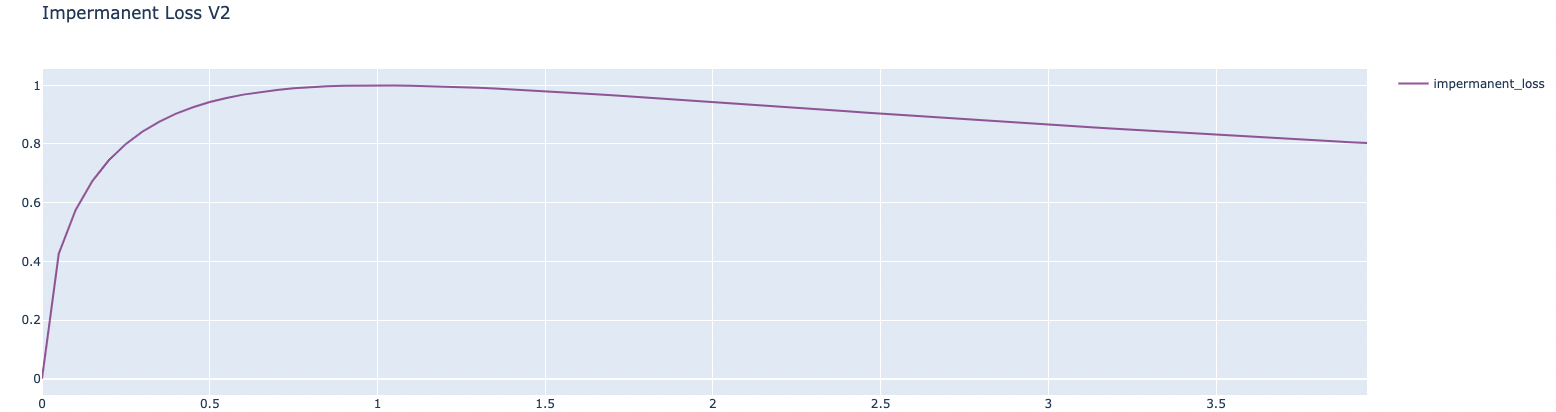
\includegraphics[scale=0.15]{Plots/impermanent_loss.png}
    \caption{Impermanent loss versus price ratio}
    \label{fig:rangy_market}
\end{figure}

\begin{description}
\item[$\bullet$1.25x price change results in a 0.6\% loss relative to HODL]
\item[$\bullet$1.50x price change results in a 2.0\% loss relative to HODL]
\item[$\bullet$1.75x price change results in a 3.8\% loss relative to HODL]
\item[$\bullet$2x price change results in a 5.7\% loss relative to HODL]
\item[$\bullet$3x price change results in a 13.4\% loss relative to HODL]
\item[$\bullet$4x price change results in a 20.0\% loss relative to HODL]
\item[$\bullet$5x price change results in a 25.5\% loss relative to HODL]
\end{description}
“N.B. The loss is the same whichever direction the price change occurs in  (doubling in price results in the same loss as halving).\\

\subsection{Uniswap V3 Impermanent loss}
The idea behind Uniswap V3 is that the user can specify a price range where he wants to bring the liquidity.
\\
The price range is specified by two bounds on the risky asset price $P_a <= P_b$ and the liquidity brought by the user will only account for that range allowing a huge gain in capital efficiency.\\


\subsubsection{Capital efficiency and uniswap v3}
From now on, the only price we will deal with is the price of the risky asset in stable coin.
\begin{equation}
    P = P_X = P_{X \text{ in }Y}  = \frac{Y}{X}
\end{equation}
With that notation, it comes :
\begin{equation}
    L=\sqrt{X*Y}
\end{equation}
\begin{equation}
    X = \frac{L}{\sqrt{P}}  
\end{equation}
\begin{equation}
    Y = L*\sqrt{P}
\end{equation}
\subsubsection{ Swapping inside a tick}
Inside a tick, everything works as with the previous Uniswap V2 protocol with virtual reserves.
\begin{equation}
    X_{virtual} * Y_{virtual} = L^2
\end{equation}
And the reserves evolution are dictated by
\begin{equation}
   \Delta \sqrt{P} = \frac{\Delta Y}{L}
\end{equation}
\begin{equation}
   \Delta \frac{1}{\sqrt{P}} = \frac{\Delta X}{L}
\end{equation}
The smart contract will only track the $L$ and $\sqrt{P}$. The reserve will be updated
accordingly.

\\
The risky asset reserve matching the highest price for which the liquidity provider is ready to provide liquidity :
\begin{equation}
    X_b = \frac{L}{\sqrt{P_b}}
\end{equation}
The stable coin reserve matching the lowest price for which the liquidity provider is ready to provide liquidity :
\begin{equation}
    Y_a = L *\sqrt{P_a}
\end{equation}
\begin{equation}
\left\{
\begin{array}{ll}
  X_{virtual} = X_{real}+\frac{L}{\sqrt{P_b}}\\
  Y_{virtual} = Y_{real} + L *\sqrt{P_a}\\
\end{array}
\right.
\end{equation}
The hyperbole equation thus becomes:
\begin{equation}
    (X_{real}+\frac{L}{\sqrt{P_b}})* (Y_{real} + L *\sqrt{P_a})= L^2
\end{equation}
From now on, we will give up the real tag and call $X=X_{real}$ and $Y=Y_{real}$.
%For $P\ge P_b$:
%\begin{equation}
%\left\{
%\begin{array}{ll}
%X=0\\
%Y=L*(\sqrt{P_b}-\sqrt{P_a})\\
%\end{array}
%\right.
%\end{equation}
%\\
%For $P\le P_a$:
%\begin{equation}
%\left\{
%\begin{array}{ll}
%X=L*\frac{\sqrt{P_b}-\sqrt{P_a}}{\sqrt{P_b}*\sqrt{P_a}}\\
%Y=0\\
%\end{array}
%\right.
%\end{equation}
%\\
%For $P_a \le P \le P_b $:
%\begin{equation}
%\left\{
%\begin{array}{ll}
%X=X_{virtual}-\frac{L}{\sqrt{P_b}}=L*(\frac{1}{\sqrt{P}}-\frac{1}{\sqrt{P_b}}) %=L*\frac{\sqrt{P_b}-\sqrt{P}}{\sqrt{P_b}*\sqrt{P}}\\
%Y=Y_{virtual}-L*\sqrt{P_a}\ = L*(\sqrt{P}-\sqrt{P_a})\\
%\end{array}
%\right.
%\end{equation}
\\
The solution is given by the three different regimes according to the current price $P$ location regarding the liquidity bounds:
\begin{equation}\label{three_regime}
\left\{
\begin{array}{cc}
\begin{array}{lllll}
\left\{
\begin{array}{ll}
X=0\\
Y=L*(\sqrt{P_b}-\sqrt{P_a})\\
\end{array}
\right. & ,P\ge P_b\\
& \\
\left\{
\begin{array}{ll}
X=L*(\frac{1}{\sqrt{P}}-\frac{1}{\sqrt{P_b}}) \\
Y= L*(\sqrt{P}-\sqrt{P_a})\\
\end{array}
\right.&  ,P_a \le P \le P_b \\
&\\
\left\{
\begin{array}{ll}
X=L*(\frac{1}{\sqrt{P_a}}-\frac{1}{\sqrt{P_b}})\\
Y=0\\
\end{array}
\right.& ,P\le P_a\\
\end{array}
\right.\\
\end{array}
\end{equation}

\begin{figure}[h!]
    \centering
    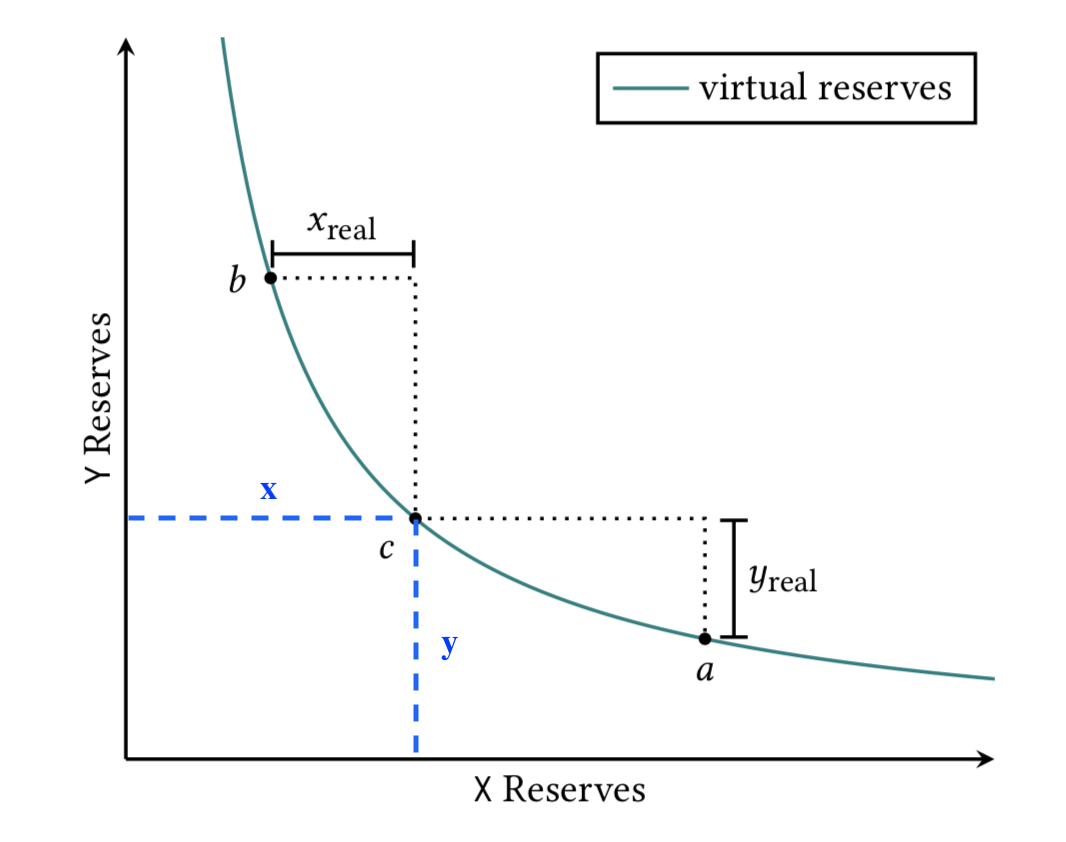
\includegraphics[scale=0.2]{Plots/concentrated_liquidity.png}
    \caption{Concentrated liquidity between a and b}
    \label{fig:conc_liquidity}
\end{figure}
\subsection{Computing the impermanent loss}
The value of the pool at a time $t$ when the pool is arbitraged :
\begin{equation}
V=X*P+Y\\
\end{equation}
$$
V = L*( \frac{1}{\sqrt{P}}-\frac{1}{\sqrt{P_b}})*P + L*(\sqrt{P}-\sqrt{P_a})
$$
\begin{equation}
V = 2*L*\sqrt{P}-L*(\sqrt{P_a}+ \frac{P}{\sqrt{P_b}}})
\end{equation}

Let's define $P_{consensus}$, the new price coming from a market consensus and $\tau>0$ the price ratio.
\begin{equation}
P_{consensus} = \tau*P\\
\end{equation}

The value of the arbitraged pool with the new consensus price is then :
\begin{equation}
V_{arbitraged} = 2*L*\sqrt{\tau*P}-L*(\sqrt{P_a}+ \frac{\tau*P}{\sqrt{P_b}}} )
\end{equation}

\begin{equation}
V_{held} = X*P_{consensus}+Y
\end{equation}
$$
V_{held} = L*( \frac{1}{\sqrt{P}}-\frac{1}{\sqrt{P_b}})*P_{consensus}+L*(\sqrt{P}-\sqrt{P_a})+ \\
$$

$$
V_{held} = L*\sqrt{P}*(1+\tau)-L*(\sqrt{P_a}+ \frac{\tau*P}{\sqrt{P_b}}})\\
$$
The V3 impermanent loss is thus after a quick computation :
\begin{equation}\label{eq:ILv3}
\frac{V_{arbitraged} - V_{held}}{V_{held}} = 
IL_{v2}(\tau)*\frac{1}{1 -\frac{ \sqrt{\frac{P_a}{P}} + \tau*\sqrt{\frac{P}{P_b}}} { 1+\tau}}} = IL_{P_a,P_b}(\tau)
\end{equation}
where $IL_{v2}(\tau)=\frac{2*\sqrt{\tau}}{1+\tau}}-1 = IL_{v2}(\tau)$ is the standard uniswap V2 impermanent loss for the range $\left[0,+\infty\right[$.\\
In the case $P_a = P_b = P$, then the impermanent loss will be $0$.
\begin{equation}
\lim\limits_{P_a \to 0, P_b \to +\infty} IL_{P_a,P_b}(\tau) = IL(\tau)
\end{equation}
When the liquidity bounds are pushed to $[0,+\infty[$, the $v3$ impermanent loss goes back to the original v2 one.\\
 
Finally, setting $\tau$ to 1, we do get 0 since there should not be any impermanent loss in any scenario, v2 or v3.\\
\subsubsection{V3 Impermanent loss is larger}

If we take the simple assumption $p_a = \frac{P}{n}$ and $p_b = n*P$, we get the following loss :
\begin{equation}\label{nasty_il}
IL_{P_a,P_b}(\tau) = IL(\tau) * \frac{1}{1-\frac{1}{\sqrt{n}}}
\end{equation}
\begin{figure}[h!]
    \centering
    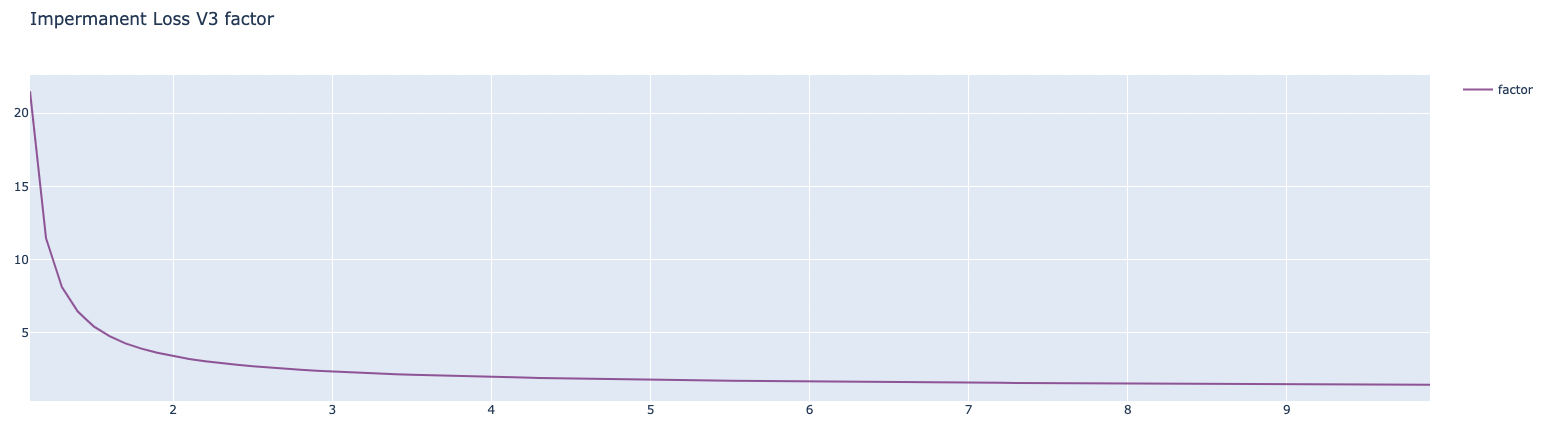
\includegraphics[scale=0.15]{Plots/factor.png}
    \caption{Impermanent loss V3 factor}
    \label{fig:rangy_market}
\end{figure}

Even if our liquidity range is big enough to accommodate prices doubling or halving, impermanent loss is nearly 4 times higher than if we provided liquidity in the whole range of prices.\\
And that is excluding the impermanent loss associated with falling outside the concentrated liquidity range.\\
\subsection{Uniswap V3 LP liquidity providing value}
\subsubsection{Add/deletion of liquidity}
When adding or removing liquidity from a position, the amount of assets to add according to the amount of added liquidity $\Delta L$
is given by the equivalent formula as \ref{three_regime}:
\begin{equation}\label{liquidity_adding}
\left\{
\begin{array}{cc}
\begin{array}{lllll}
\left\{
\begin{array}{ll}
\Delta X=0\\
\Delta Y=\Delta L*(\sqrt{P_b}-\sqrt{P_a})\\
\end{array}
\right. & ,P\ge P_b\\
& \\
\left\{
\begin{array}{ll}
\Delta X=\Delta L*(\frac{1}{\sqrt{P}}-\frac{1}{\sqrt{P_b}}) \\
\Delta Y= \Delta L*(\sqrt{P}-\sqrt{P_a})\\
\end{array}
\right.&  ,P_a \le P \le P_b \\
&\\
\left\{
\begin{array}{ll}
\Delta X=\Delta L*(\frac{1}{\sqrt{P_a}}-\frac{1}{\sqrt{P_b}})\\
\Delta Y=0\\
\end{array}
\right.& ,P\le P_a\\
\end{array}
\right.\\
\end{array}
\end{equation}
\subsubsection{Valuing a liquidity position}
The initial amount of tokens $X_0$, $Y_0$ and $L$ when entering a LP position with bounds $P_a$ and $P_b$ and initial price $P_0$ will follow \ref{three_regime}.\\
You can deduct $L$ value from \ref{three_regime} applied to $X_0$, $Y_0$ and $P_0$.\\
The final amount of tokens $X$, $Y$ and $L$ when exiting a LP position with bounds $P_a$ and $P_b$ and current price $P$ will also follow \ref{three_regime} for the previous $L$.\\
The liquidity position P&L can be written as :
\begin{equation}\label{PnL}
PnL = \frac{X* P + Y}{X_0 * P_0 + Y_0} - 1
\end{equation}

\section{Actively monitoring your liquidity}
\subsection{Encompassing the market by defining bounds from the Bollinger Bands}
The idea behind Uniswap V3 is that the user can specify a price range where he wants to bring the liquidity.
\\
The price range is specified by two bounds on the risky asset price $P_a <= P_b$ and the liquidity brought by the user will only account for that range allowing a huge gain in capital efficiency.\\
The tighter the bounds, the more efficient the liquidity capital is, but the more you will have to rebalance and incur impermanent loss and swapping costs.\\
Bollinger Bands are a type of price envelopes plotted at a standard deviation level above and below a simple moving average of the price. Because the distance of the bands is based on standard deviation, they adjust to volatility swings in the underlying price.\\
Bollinger Bands use 2 parameters, the 'Period' parameter T for the moving average and n or the number of standard deviations $\sigma$. \\
Bollinger bands help determine whether prices are high or low on a relative basis. They are used in pairs, both upper and lower bands and in conjunction with a moving average. Further, the pair of bands is not intended to be used on its own. Use the pair to confirm signals given with other indicators.\\
We will use Bollinger bands to define our liquidity price bounds at a specific rebalancing time $t$. The larger the number of standard deviations $n$, the broader the bands will get allowing a conservative liquidity range.\\
The bounds are fixed by the calibrated Bollinger band and the initial position entering $P_0$ price.
\begin{equation}
P_b = P_0 + n*\sigma
\end{equation}
\begin{equation}
P_a = P_0 - n*\sigma
\end{equation}
\begin{equation}
P_0 = \frac{P_a + P_b}{2} 
\end{equation}

\subsection{Rebalancing trigger}
If we were to rebalance each time a bound is reached, we can rewrite the v3 impermanent loss according to the strategy. \\
By noting $\kappa = \frac{P_b}{P_a} = \frac{P_0 + n*\sigma}{P_0-n*\sigma}  $, the v3 impermanent loss can be rewritten:
\begin{equation}\label{eq:ILv3Stratbis}
\frac{V_{arbitraged} - V_{held}}{V_{held}} = 
IL_{v2}(\tau)*\frac{1}{1 -\frac{ \sqrt{\frac{2}{1 +\kappa}} + \tau*\sqrt{\frac{1}{2}(1+\frac{1}{\kappa})}} { 1+\tau}}}
\end{equation}
A position is exited when one of its bound is touched, meaning that we will incur
two different IL loss depending on whether we reached the lower bound or the upper bound :
\begin{equation}
\tau_{up} = \frac{P_0}{P_0+n*\sigma}    
\end{equation}
\begin{equation}
\tau_{down} = \frac{P_0}{P_0-n*\sigma}    
\end{equation}
Equation \ref{eq:ILv3Stratbis} and its simplified version \ref{nasty_il} shows how nasty v3 impermanent loss can be for tighter bounds.\\
But one other very important thing has to be factored in : if we were to wait for a bound to be reached for rebalancing the position, we would then have to swap roughly half of our assets to enter a new position.\\
For huge AUM (asset under management) and fully on-chain rebalancing vaults, price slippages occurring during swaps can be very detrimental to the strategy.\\
AuM swapping costs are an essential part of the backtest : it will drive the optimal backtesting rebalancing parameters and will account for the asset under management scaling up : as AUM grows and swapping costs explodes, one will find optimal parameters with fewer rebalancing times.\\
We add a new parameter $\tau$, which is a number between 0 and 1. This parameter is intended to trigger a rebalancing each time we approach the upper or lower Bollinger band at a relative $\tau$ distance.\\
The trigger condition is defined by\\
\begin{equation}\label{trigger}
P \ge P_b-\tau P_b \text{ or } P \le P_a+\tau P_a  
\end{equation}
\subsection{Swapping costs}
The final asset quantities $X_f$ and $Y_f$ in the LP position can be found by using the final price $$P_f = P_b-\tau P_b \text{ or } P_f = P_a+\tau P_a $$ in equation \ref{three_regime}. Depending on whether we got triggered by the upper bound proximity or lower bound proximity, we will end up in a disequilibrium with the paroxysm reached for $\tau =0$ : then $P_f = P_b$ implicates that we are full in stable coins $Y$ and $P_f = P_a$ implicates that we are full in risky asset $X$.\\
We then have to swap part of either $X_f$ or $Y_f$ to fully reenter a position.\\

\section{Exhaustive optimization}
\subsection{Getting the optimal parameters: A trade-off between rebalancing costs, IL and generated fees}
The chosen bounds must also fit perfectly the price envelope for the optimal capital efficiency of your liquidity provisioning, while minimizing impermanent loss and swapping costs.\\
So in other words, we end up with the following constrained optimization problem :
\\
\begin{description}
  \item[$\bullet$]Maximize price inside the tightest bounds to earn volume fees (the tighter the bounds, the efficienter the capital)
  \item[$\bullet$] Impermanent loss and swapping slippage costs incurred at each rebalancing have to be minimized
\end{description}
We here propose an exhaustive search of the optimal parameters by running a backtest for each configuration and choosing the solution with the best Sharpe ratio.\\
\begin{equation}
\max_{(n, T, \tau, swap-costs)} \left[ Sharpe\left(n, T, \tau, swap-costs\right)\right]
\end{equation}
where $Sharpe\left(n, T, \tau, swap-costs\right)$ is the sharpe ratio of the backtested path.
\subsection{Simulating the fees generation}
We do use Dune Analytics to fetch the past volume $https://dune.com/queries/1343928$ and we use a rule of thumb volume pro rata to infer the past range APYs by just multiplying a snapshot of the APYs range by the pro rata of the current volume on the past one. This is a necessary approximation as we can't reproduce the whole past liquidity profile.\\

Find the average daily volume of a pool averaged over a week\\
Calculate the liquidity of a potential position for already fixed start and end points.\\
Calculate a distribution of the existing liquidity overlapping with each bucket.\\ This is similar to the views in both the flipside calculator and the liquidity view of the Uniswap analytics dashboard.\\
Use the normal distribution of the price pair (using one week of daily price movement to calculate volatility = standard deviation) to calculate the probability of the price being in each bucket. This of course makes the incorrect assumption that the past volatility will reflect the future, but hey, we gotta start somewhere. We can sum up all the buckets of the total start/end range to get an expected value for total 'liquidity coverage'.\\
Pulling everything together the calculation comes out to:\\

\begin{description}
  \item[$\bullet$ Daily Fees = Pool Volume * Pool Fee \% * Liquidity Coverage Expected Value]
  \item[$\bullet$ APY = (Daily Fees / 1000) * 365\\]
\end{description}
Finally choose the highest APY position for each pool


\subsection{Simulating the slippage}
We select the asset of minimal amount after the liquidity position triggered exit $\min\left( X_f*P_f, Y_f\right)$ and we swap the surplus $$\lvert X_f*P_f-Y_f \rvert$$ of $X_f$ or $Y_f$.\\
We choose to apply conservative swapping slippage costs as a map of the percentage size of AUM to swap. The map has been calibrated through as snapshot of the worst incurred slippage for a 1 million AUM for the chosen pair. \\
$$
swapping-cost-map=
$$
$$
\left\{1:10*1e-4,5:50*1e-4,10:0.01,
$$
$$
\left 50:0.05,75:0.07,100:0.08 \right\}
$$

\section{Results}\label{result}
We here present the optimal parameters for a 95 days backtest (largest historical volume period available for Orca).\\
The optimal parameters chosen are :
\begin{equation}
\left\{\begin{array}{lll}
T = 10\\
n = 3.5\\
\tau = 10.\\
\end{array}
\right.
\end{equation}
\subsection{Absolute performance}
\begin{figure}[h!]
    \centering
    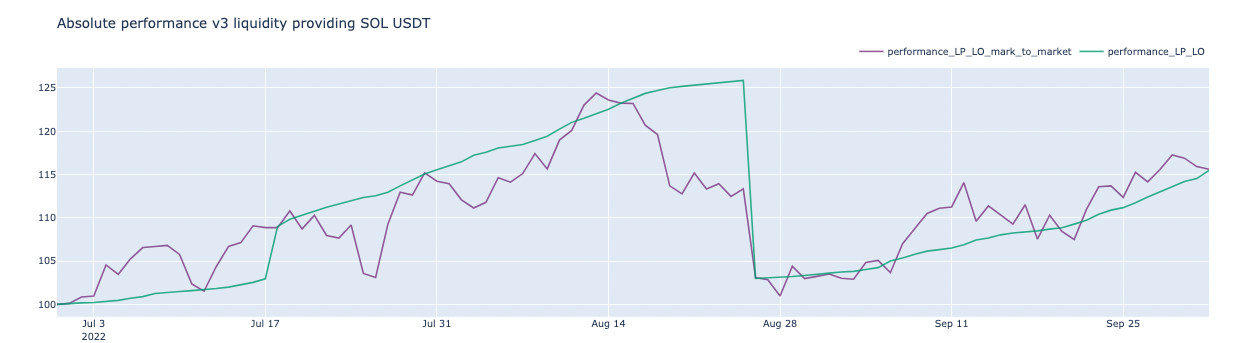
\includegraphics[scale=0.2]{Plots/absolute_lp_perf.png}
    \caption{Absolute performance}
    \label{fig:conc_liquidity}
\end{figure}
We here plot the absolute performance of the strategy against the stable coin. We have taken two approaches : one marking to market the LP value position according to the assets ratio, one just accounting for the LP value PnL at the rebalancing times. This allows to clearly demonstrate the impact of generated fees against cumulated rebalancing costs (impermanent loss, lp risky part depreciation and swapping costs).\\
We here remark that rebalancing P&L can be positive as we are in absolute performance, meaning that the LP risky asset appreciation has overtaken over impermanent loss and swap costs.
\subsection{Relative performance against 50/50 HODL basket}
\begin{figure}[h!]
    \centering
    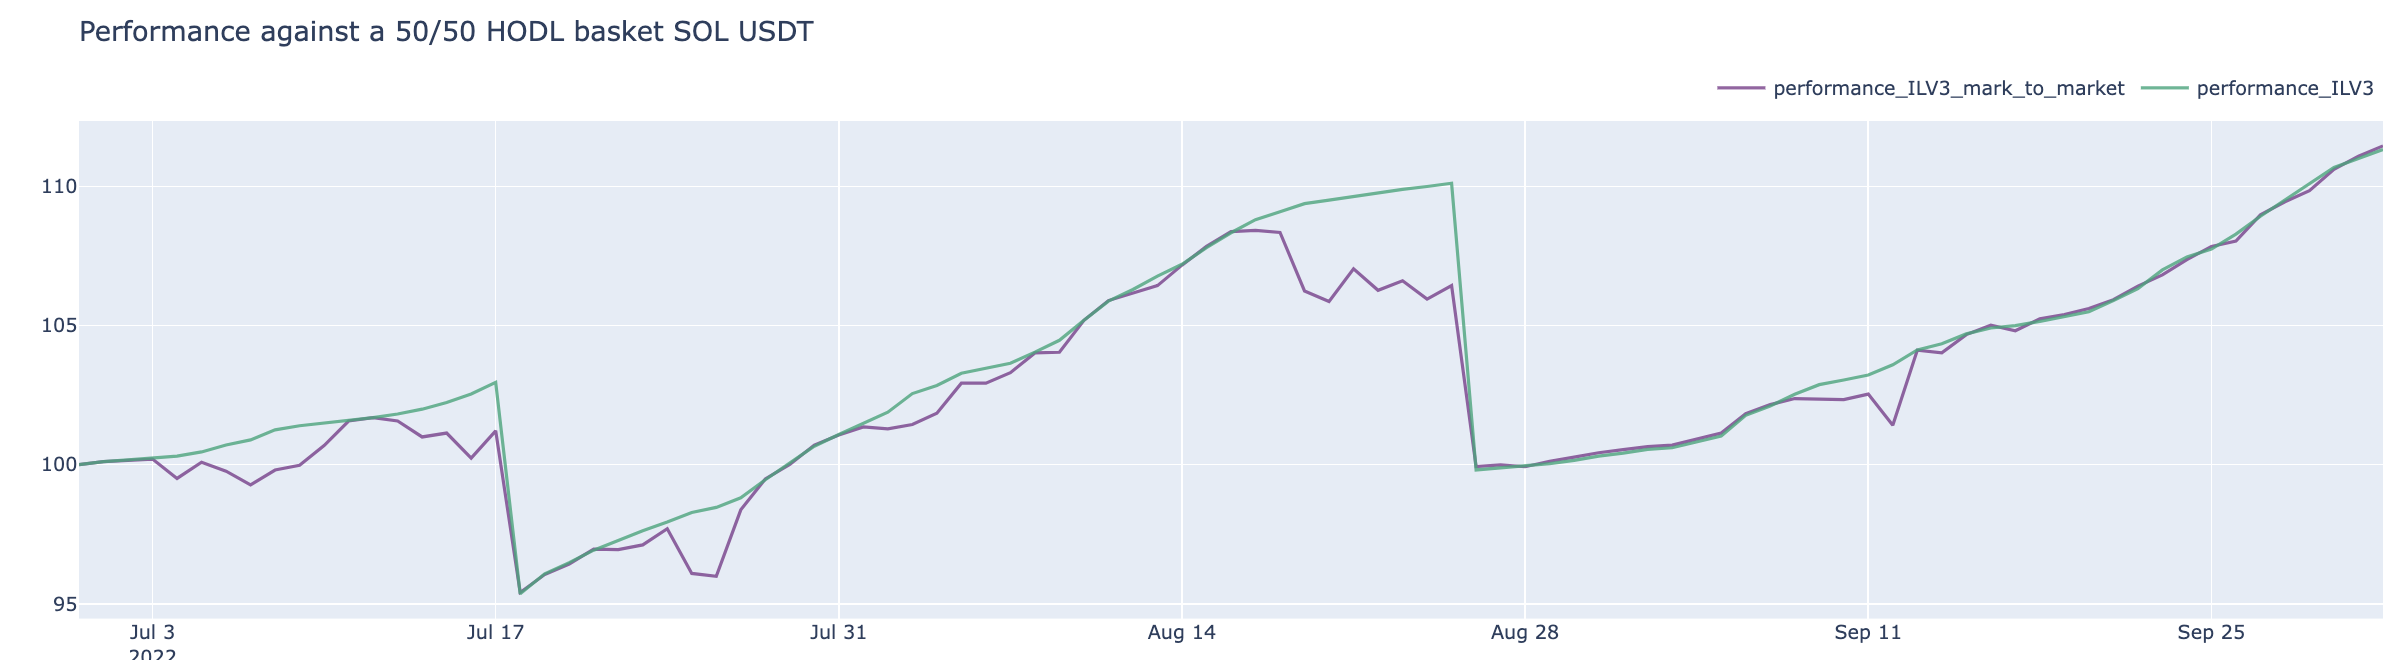
\includegraphics[scale=0.2]{Plots/hodl.png}
    \caption{Performance against a HODL basket}
    \label{fig:conc_liquidity}
\end{figure}
We here plot the relative performance of the strategy against a 50/50 HODL basket. We have taken two approaches : one marking to market the LP value position according to the assets ratio, one just accounting for the LP value PnL at the rebalancing times. This allows to clearly demonstrate the impact of generated fees against cumulated rebalancing costs (impermanent loss and swapping costs).\\
We here remark that rebalancing P&L can only be negative as impermanent loss will lose on both risky asset price increase and decrease.
\subsection{Relative performance against risky asset}
\begin{figure}[h!]
    \centering
    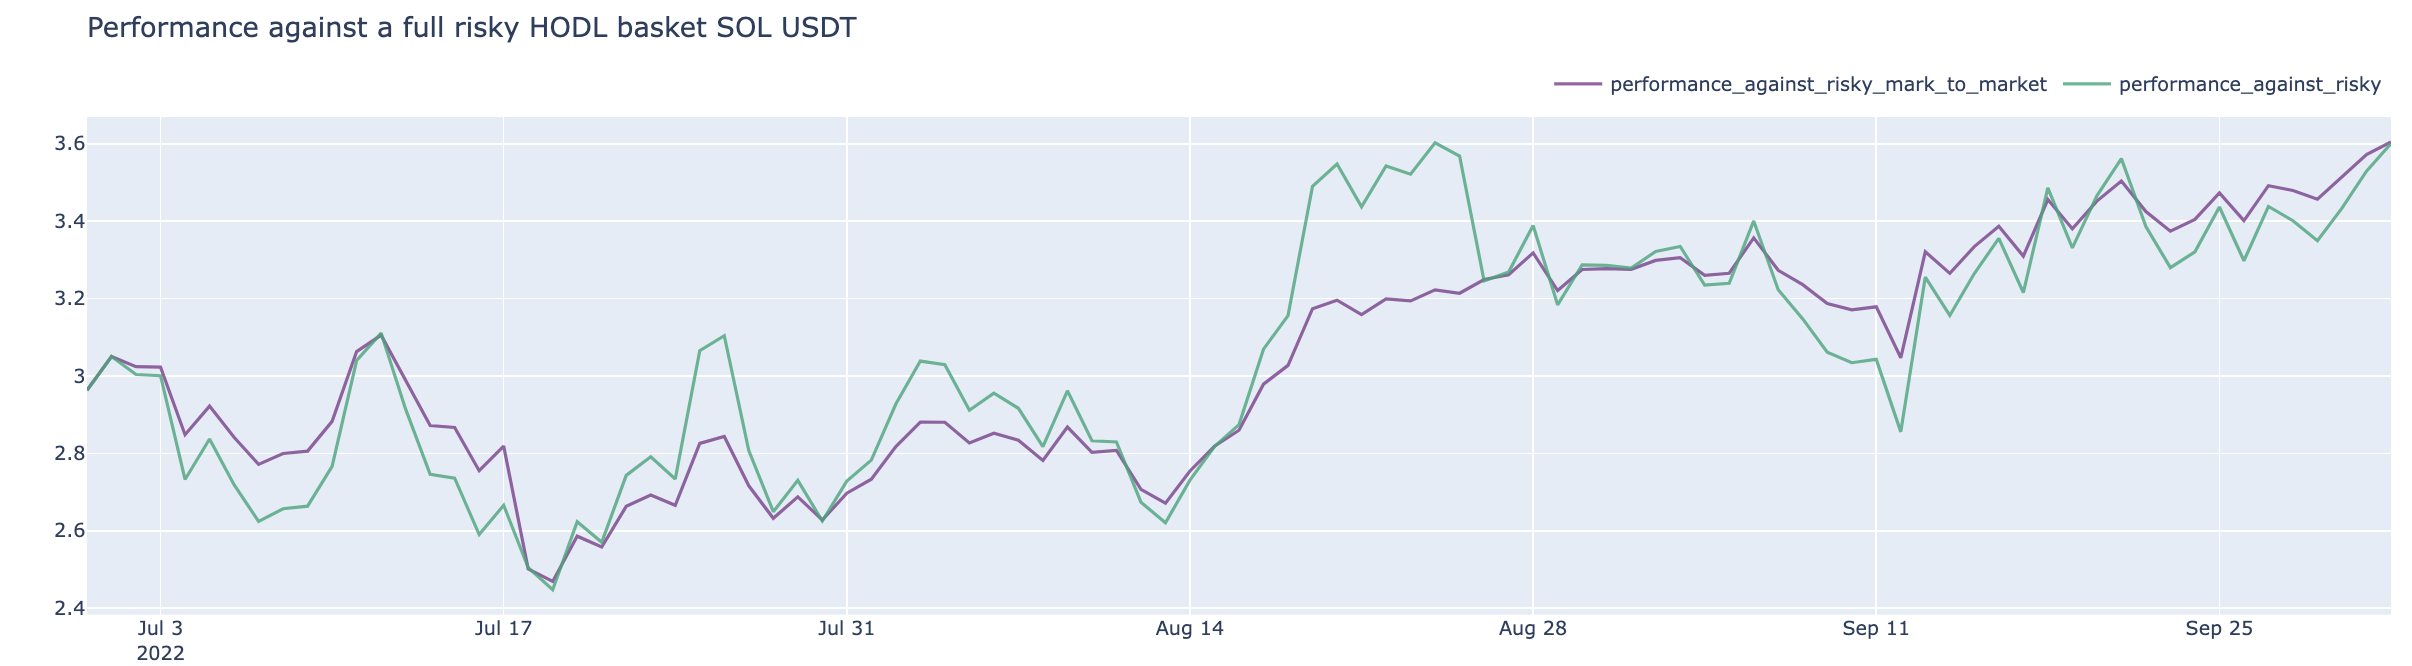
\includegraphics[scale=0.2]{Plots/risky.png}
    \caption{Performance against a full risky allocation}
    \label{fig:conc_liquidity}
\end{figure}
We here plot the relative performance of the strategy against a full risky asset allocation. We have taken two approaches : one marking to market the LP value position according to the assets ratio, one just accounting for the LP value PnL at the rebalancing times. This allows to clearly demonstrate the impact of generated fees against cumulated rebalancing costs (impermanent loss and swapping costs).\\
This approach does favour the risky asset bear price move, as the LP position is buffering a part of it with cash, and therefore the good appreciation recently.\\
\subsection{Other variable}
\subsubsection{Algorithm optimal parameters}
We here display the Bollinger bands for the optimal parameters :
\begin{figure}[h!]
    \centering
    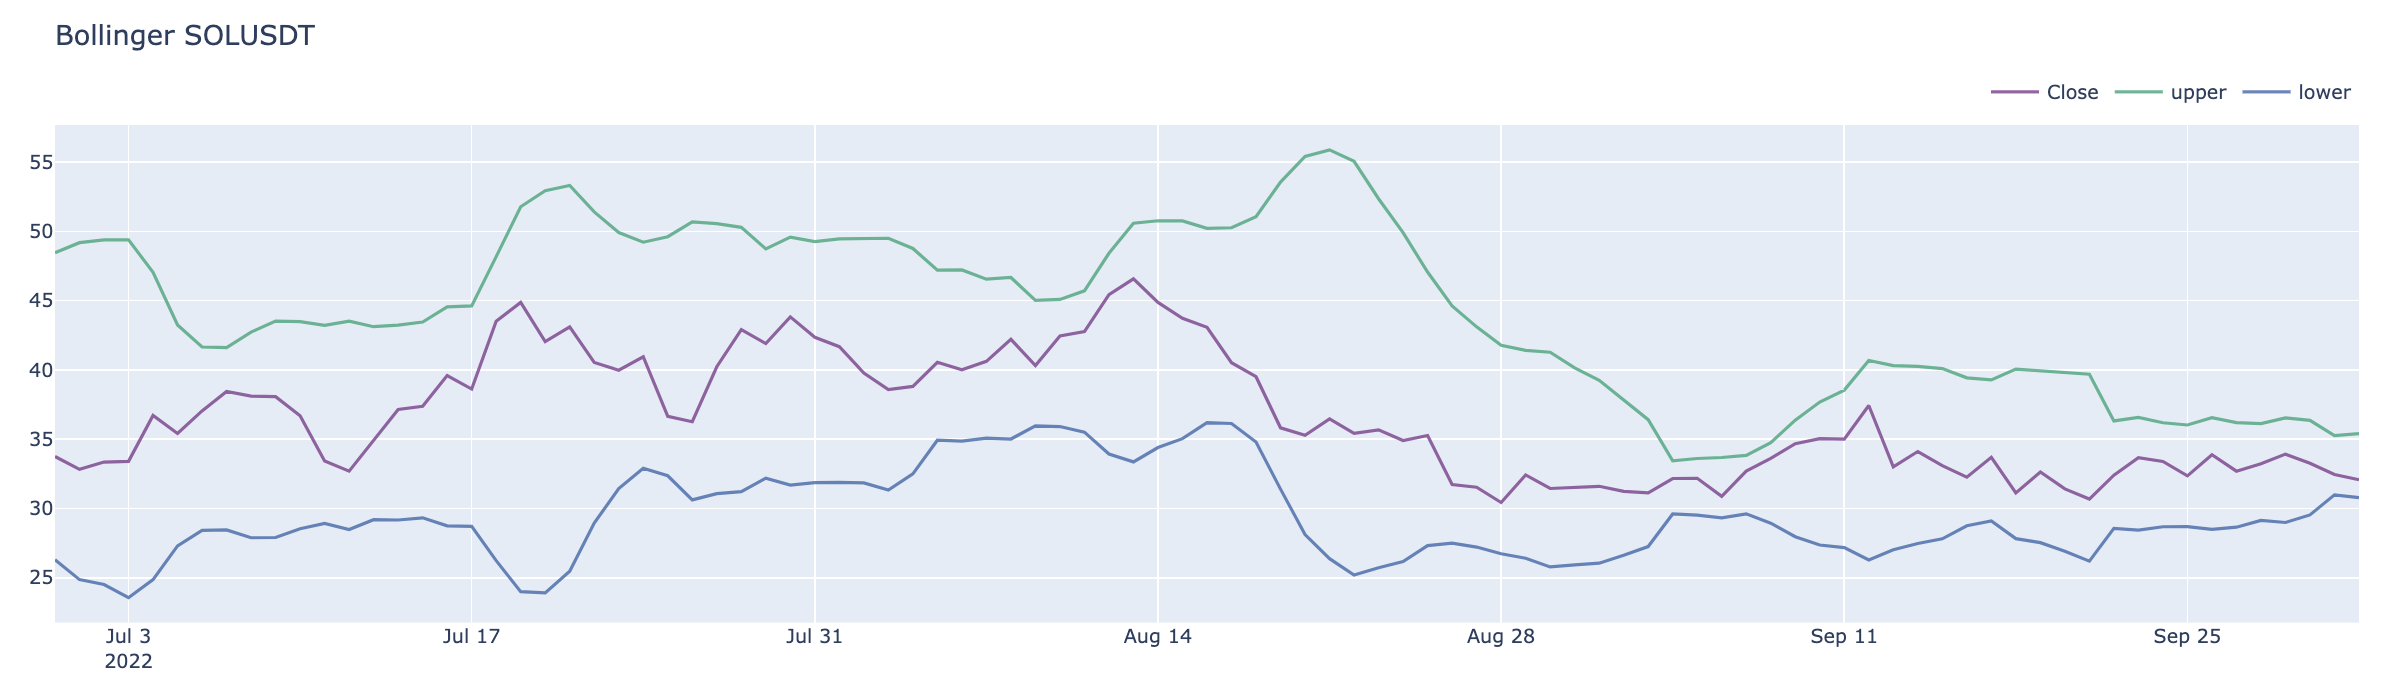
\includegraphics[scale=0.2]{Plots/bollinger.png}
    \caption{Bollinger bands}
    \label{fig:conc_liquidity}
\end{figure}
And the following derived bounds:
\begin{figure}[h!]
    \centering
    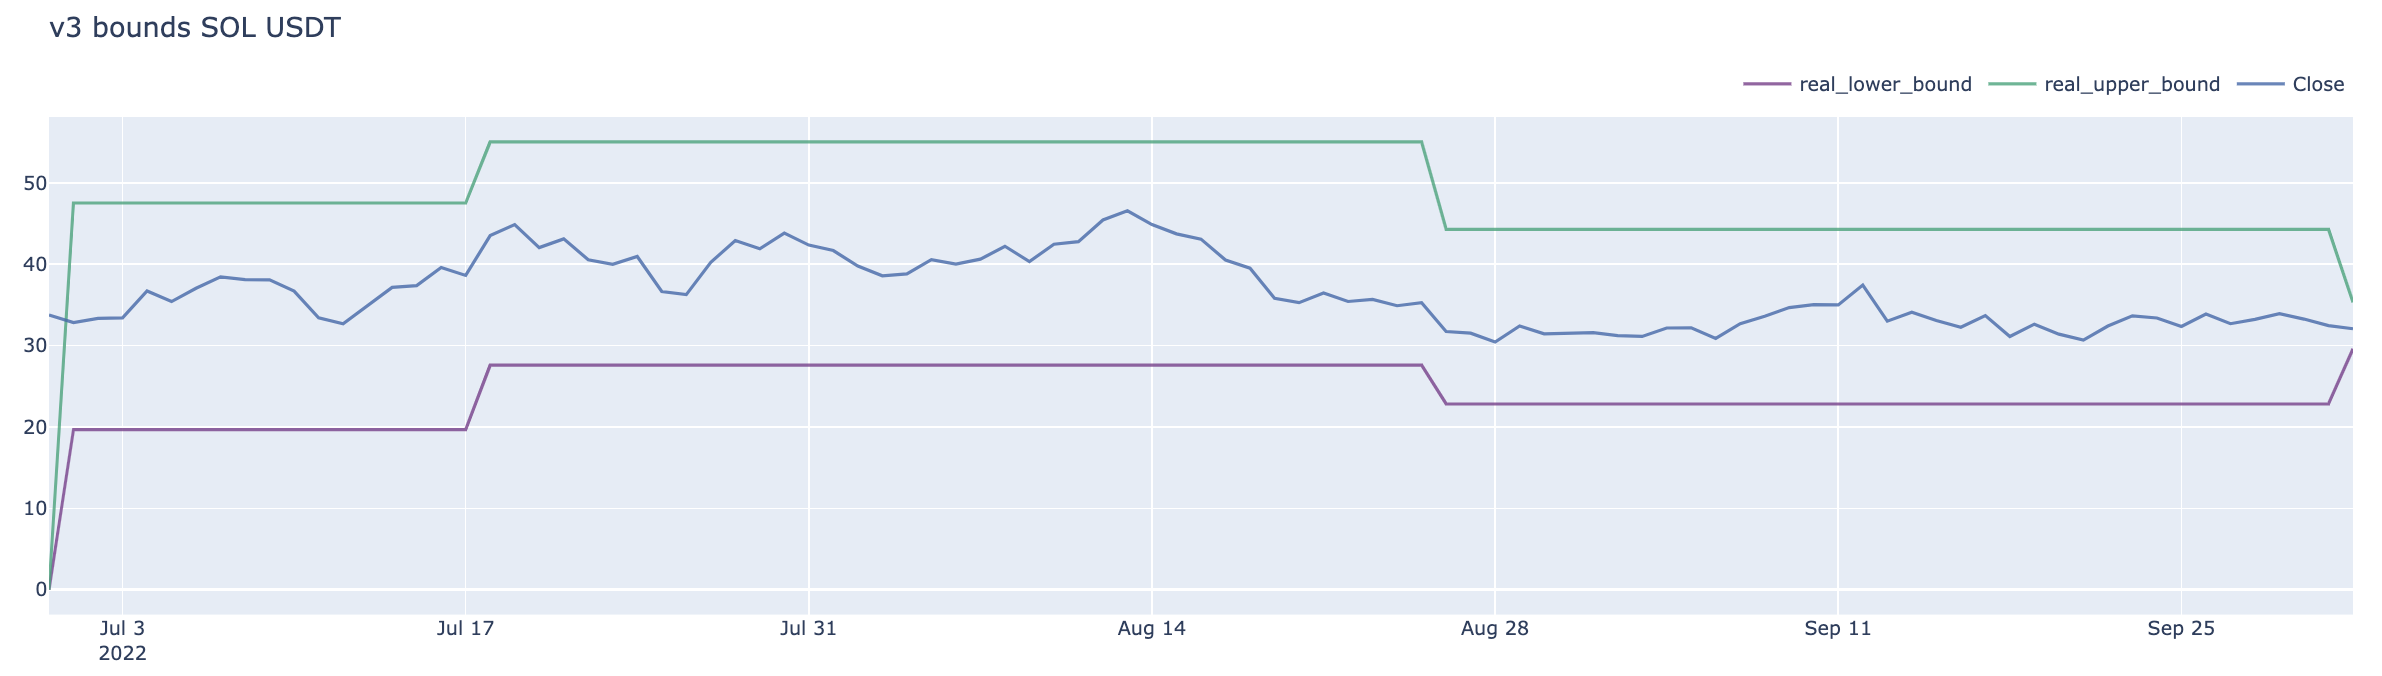
\includegraphics[scale=0.2]{Plots/bounds_over_time.png}
    \caption{Liquidity bounds}
    \label{fig:conc_liquidity}
\end{figure}
\subsubsection{Swapping costs}
The swapping costs losses computed at each rebalancing time:
\begin{figure}[h!]
    \centering
    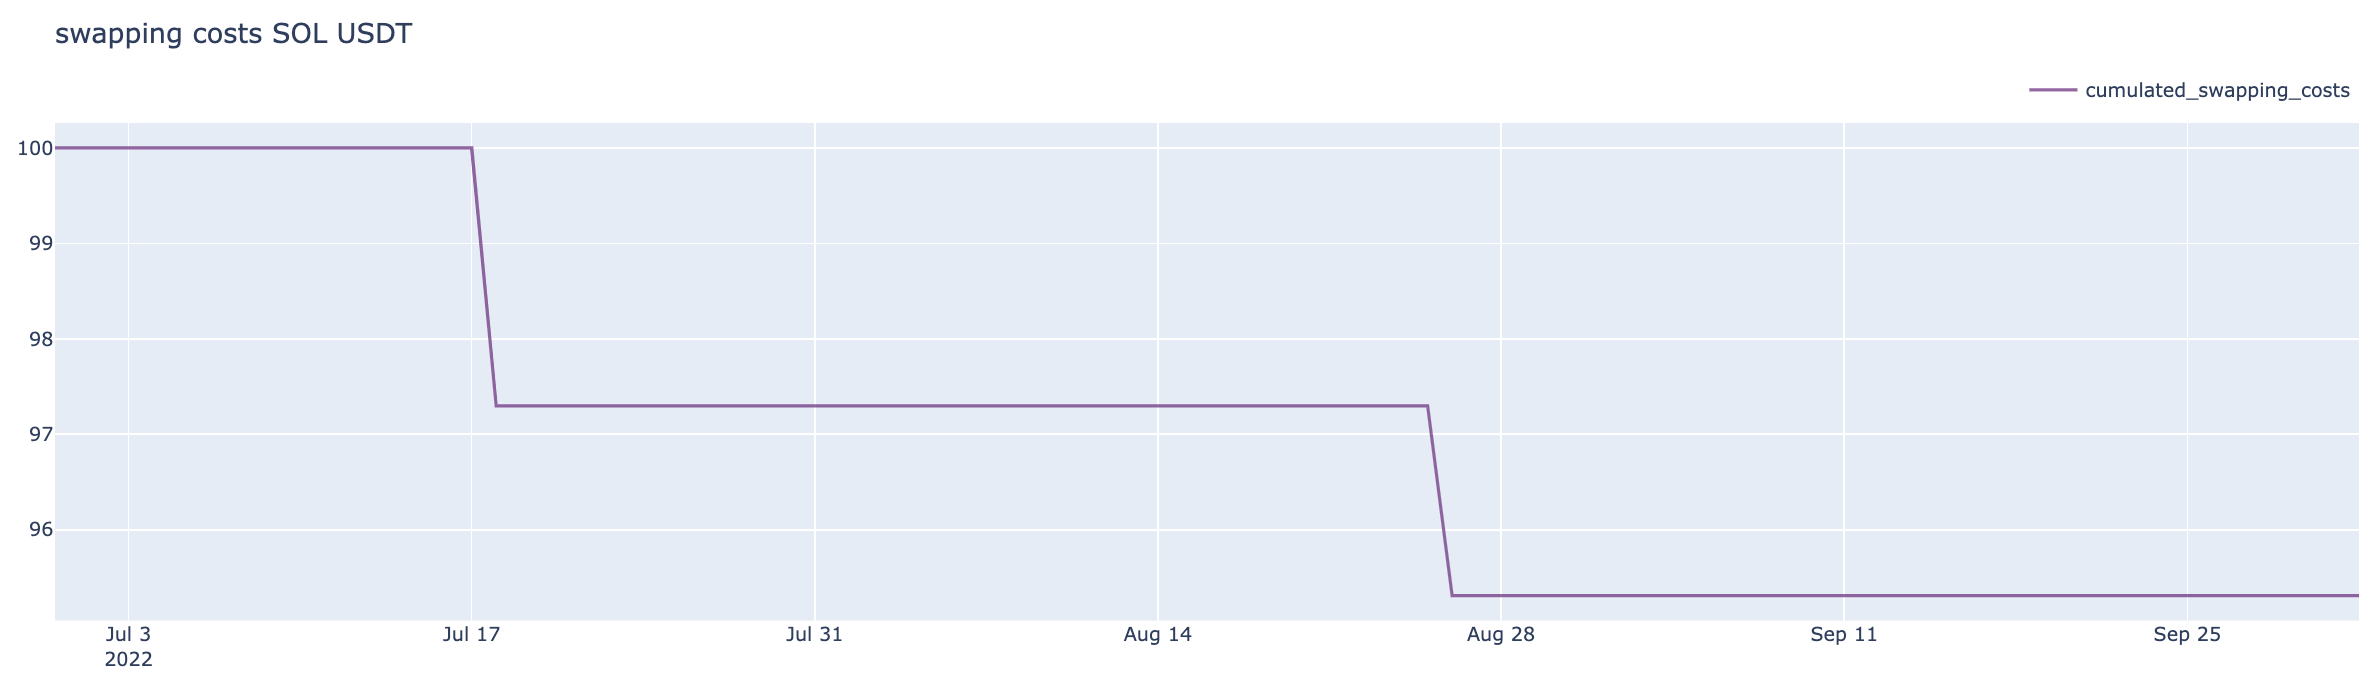
\includegraphics[scale=0.2]{Plots/swapping_cost.png}
    \caption{Swapping costs}
    \label{fig:conc_liquidity}
\end{figure}
\subsubsection{Assets proportion over time}
We give also the assets proportion in the Liquidity position. Numeraire is the non risky stable asset. Here under is his evolution over time:
\begin{figure}[h!]
    \centering
    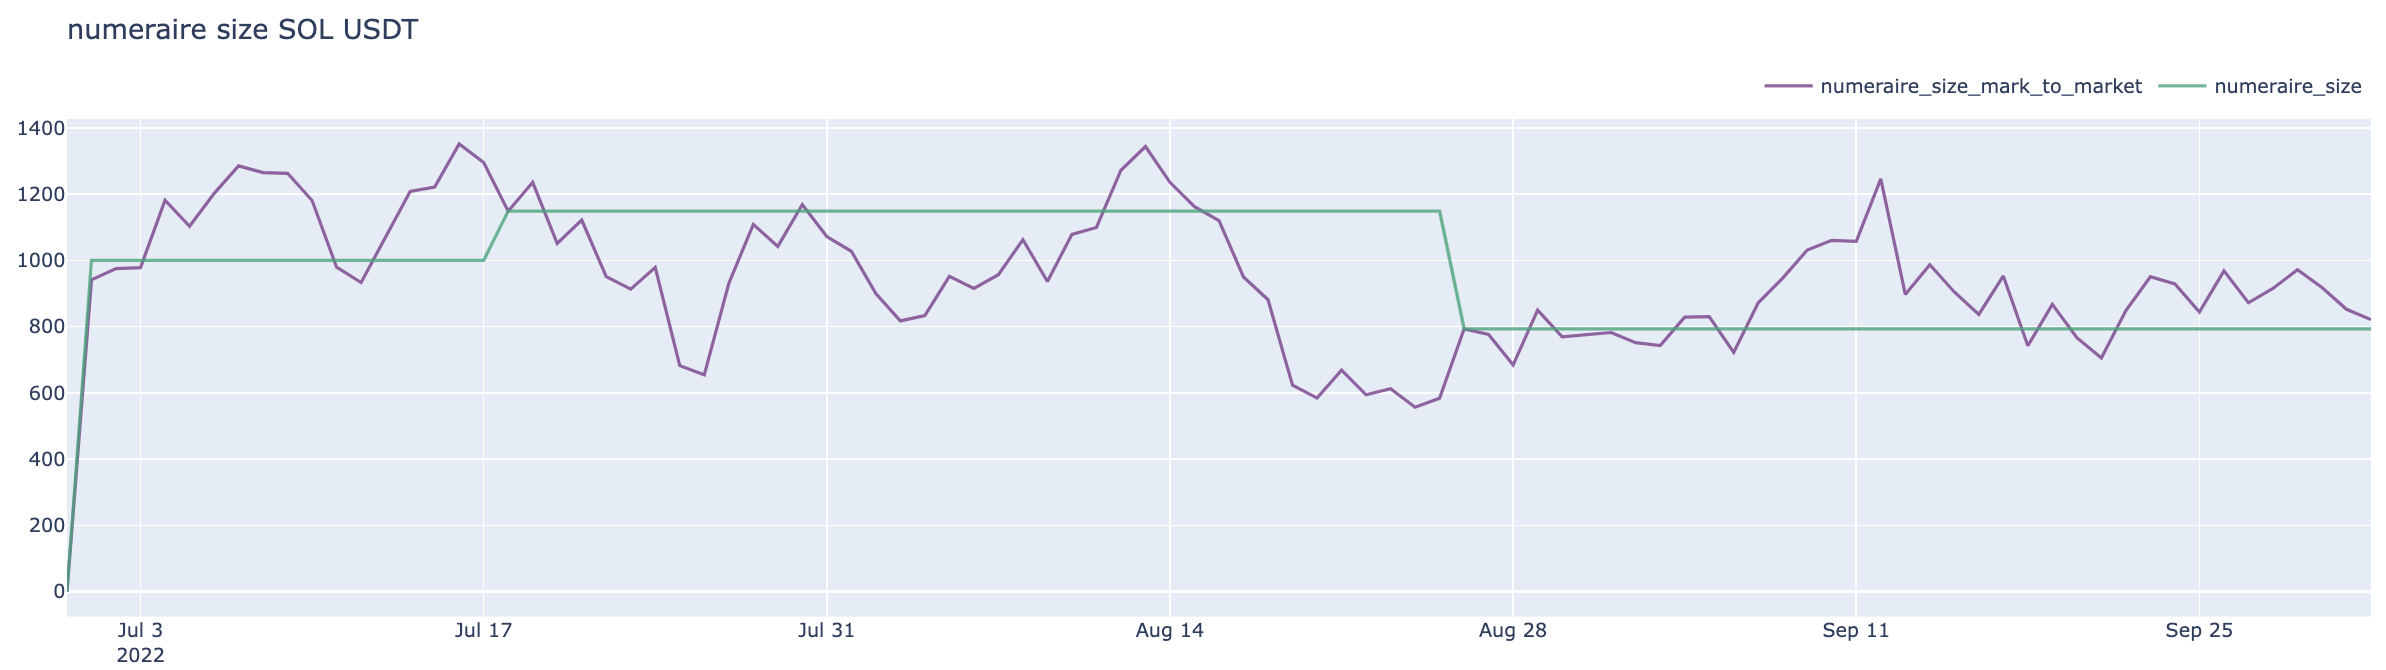
\includegraphics[scale=0.2]{Plots/numeraire_over_time.png}
    \caption{Numeraire over time}
    \label{fig:conc_liquidity}
\end{figure}
Risky asset over time:
\begin{figure}[h!]
    \centering
    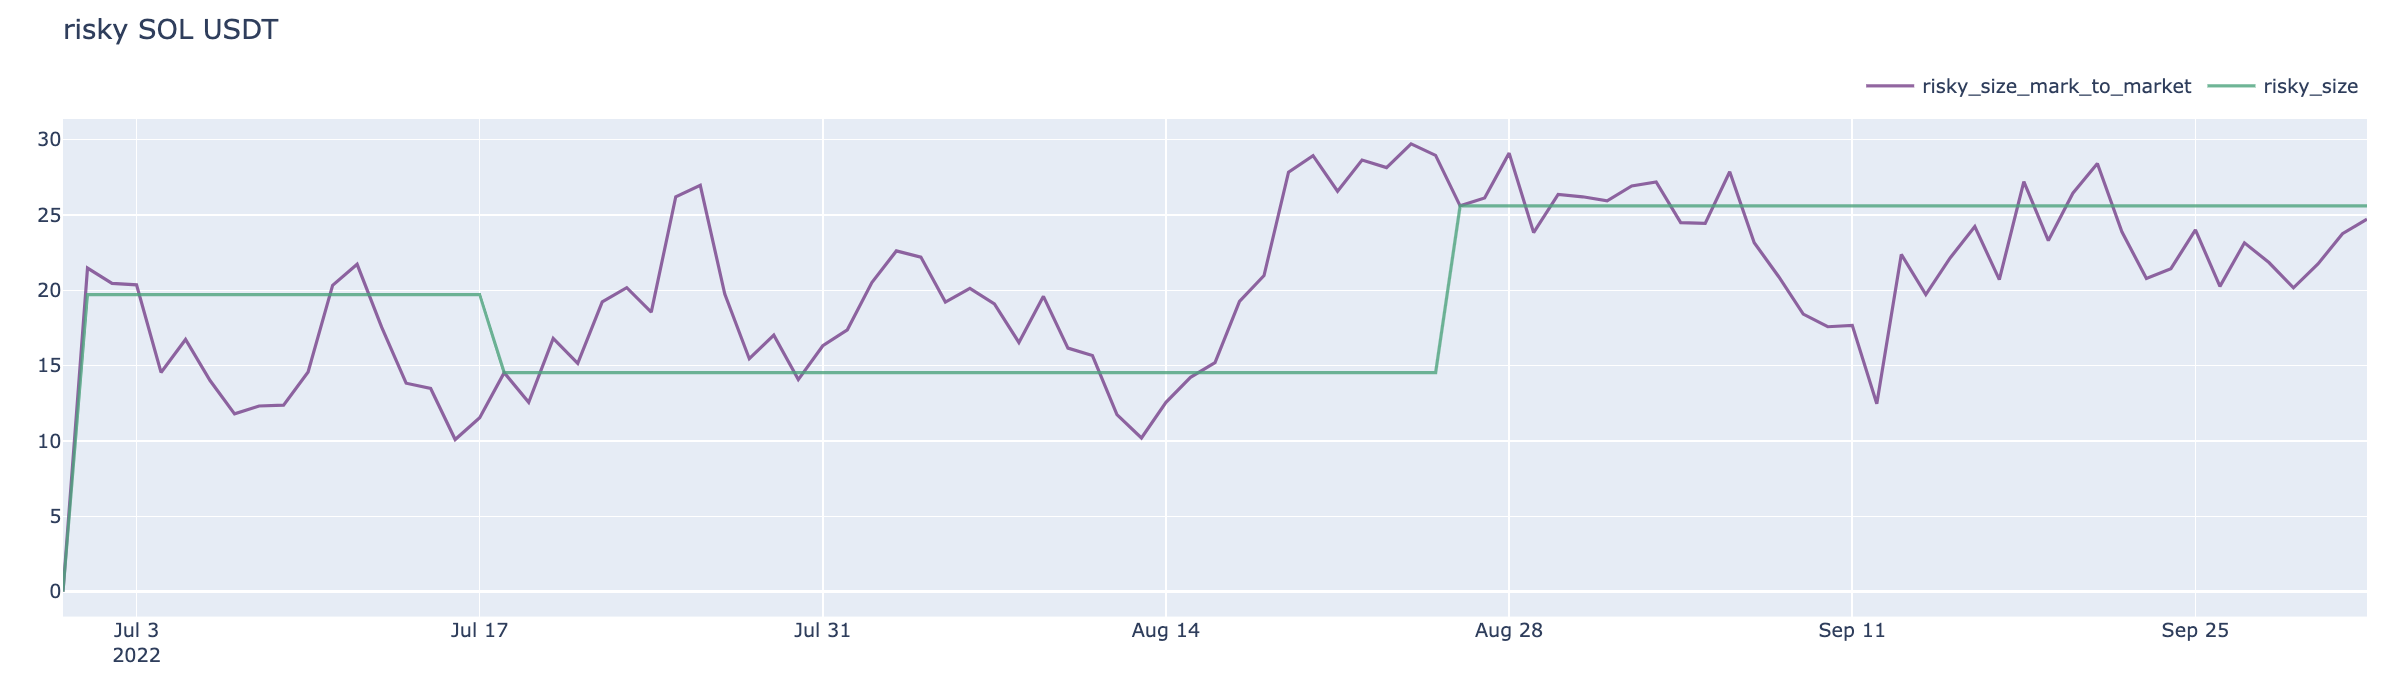
\includegraphics[scale=0.2]{Plots/risky_over_time.png}
    \caption{Risky asset over time}
    \label{fig:conc_liquidity}
\end{figure}
\subsubsection{Sensitivity analysis}
We here give financial standard kpis around the optimal parameters.\\\\
\\

\begin{tabular}{rrrrrrr}
\toprule
 T &   N &  tau &  annual\_return &  sharpe &  calmar &  mdd \\
\midrule
10 & 3.4 & 11.0 &           0.99 &    2.67 &    6.10 & 0.16 \\
11 & 3.4 & 10.0 &           0.92 &    2.48 &    5.63 & 0.16 \\
11 & 3.5 & 11.0 &           0.90 &    2.43 &    5.51 & 0.16 \\
11 & 3.6 & 11.0 &           0.88 &    2.38 &    5.39 & 0.16 \\
 9 & 3.6 &  9.0 &           0.79 &    1.99 &    4.19 & 0.19 \\
10 & 3.4 &  9.0 &           0.77 &    1.92 &    4.04 & 0.19 \\
10 & 3.4 & 10.0 &           0.77 &    1.92 &    4.04 & 0.19 \\
10 & 3.5 & 11.0 &           0.75 &    1.88 &    3.96 & 0.19 \\
10 & 3.5 &  9.0 &           0.75 &    1.88 &    3.96 & 0.19 \\
10 & 3.5 & 10.0 &           0.75 &    1.88 &    3.96 & 0.19 \\
11 & 3.4 &  9.0 &           0.73 &    1.86 &    3.93 & 0.19 \\
10 & 3.6 & 10.0 &           0.73 &    1.85 &    3.88 & 0.19 \\
10 & 3.6 & 11.0 &           0.73 &    1.85 &    3.88 & 0.19 \\
10 & 3.6 &  9.0 &           0.73 &    1.85 &    3.88 & 0.19 \\
11 & 3.5 &  9.0 &           0.71 &    1.83 &    3.85 & 0.19 \\
11 & 3.5 & 10.0 &           0.71 &    1.83 &    3.85 & 0.19 \\
11 & 3.6 & 10.0 &           0.69 &    1.79 &    3.77 & 0.18 \\
11 & 3.6 &  9.0 &           0.69 &    1.79 &    3.77 & 0.18 \\
 9 & 3.5 & 10.0 &           0.57 &    1.41 &    2.97 & 0.19 \\
 9 & 3.4 &  9.0 &          -0.24 &   -0.53 &   -0.92 & 0.25 \\
 9 & 3.5 &  9.0 &          -0.23 &   -0.53 &   -0.93 & 0.25 \\
 9 & 3.6 & 10.0 &          -0.37 &   -0.83 &   -1.27 & 0.29 \\
 9 & 3.6 & 11.0 &          -0.47 &   -1.07 &   -1.47 & 0.32 \\
 9 & 3.5 & 11.0 &          -0.47 &   -1.07 &   -1.47 & 0.32 \\
 9 & 3.4 & 10.0 &          -0.48 &   -1.08 &   -1.47 & 0.33 \\
 9 & 3.4 & 11.0 &          -0.55 &   -1.22 &   -1.57 & 0.35 \\
11 & 3.4 & 11.0 &          -0.61 &   -1.29 &   -1.68 & 0.36 \\
\bottomrule
\end{tabular}
\section{Hedging the position}
The \ref{result} results section clearly expose that the biggest losses for that strategy in absolute performance are when the risky underlying price drops. If it drops enough to trigger a rebalancing, then we have a concurrence of impermanent loss, risky asset depreciation and swapping costs which can ruin multiple months of fees generation.\\
We therefore here propose to modulate the strategy by using proprietary trend following forecasting indicator to give a downside risk level for the epoch to come.\\
According to that indicator, we here under propose two different methodologies.

\subsection{Neutral leg}
todo : copy robo vault
\subsection{Long/Short legs}
\subsubsection{Long leg}
\begin{figure}[h!]
    \centering
    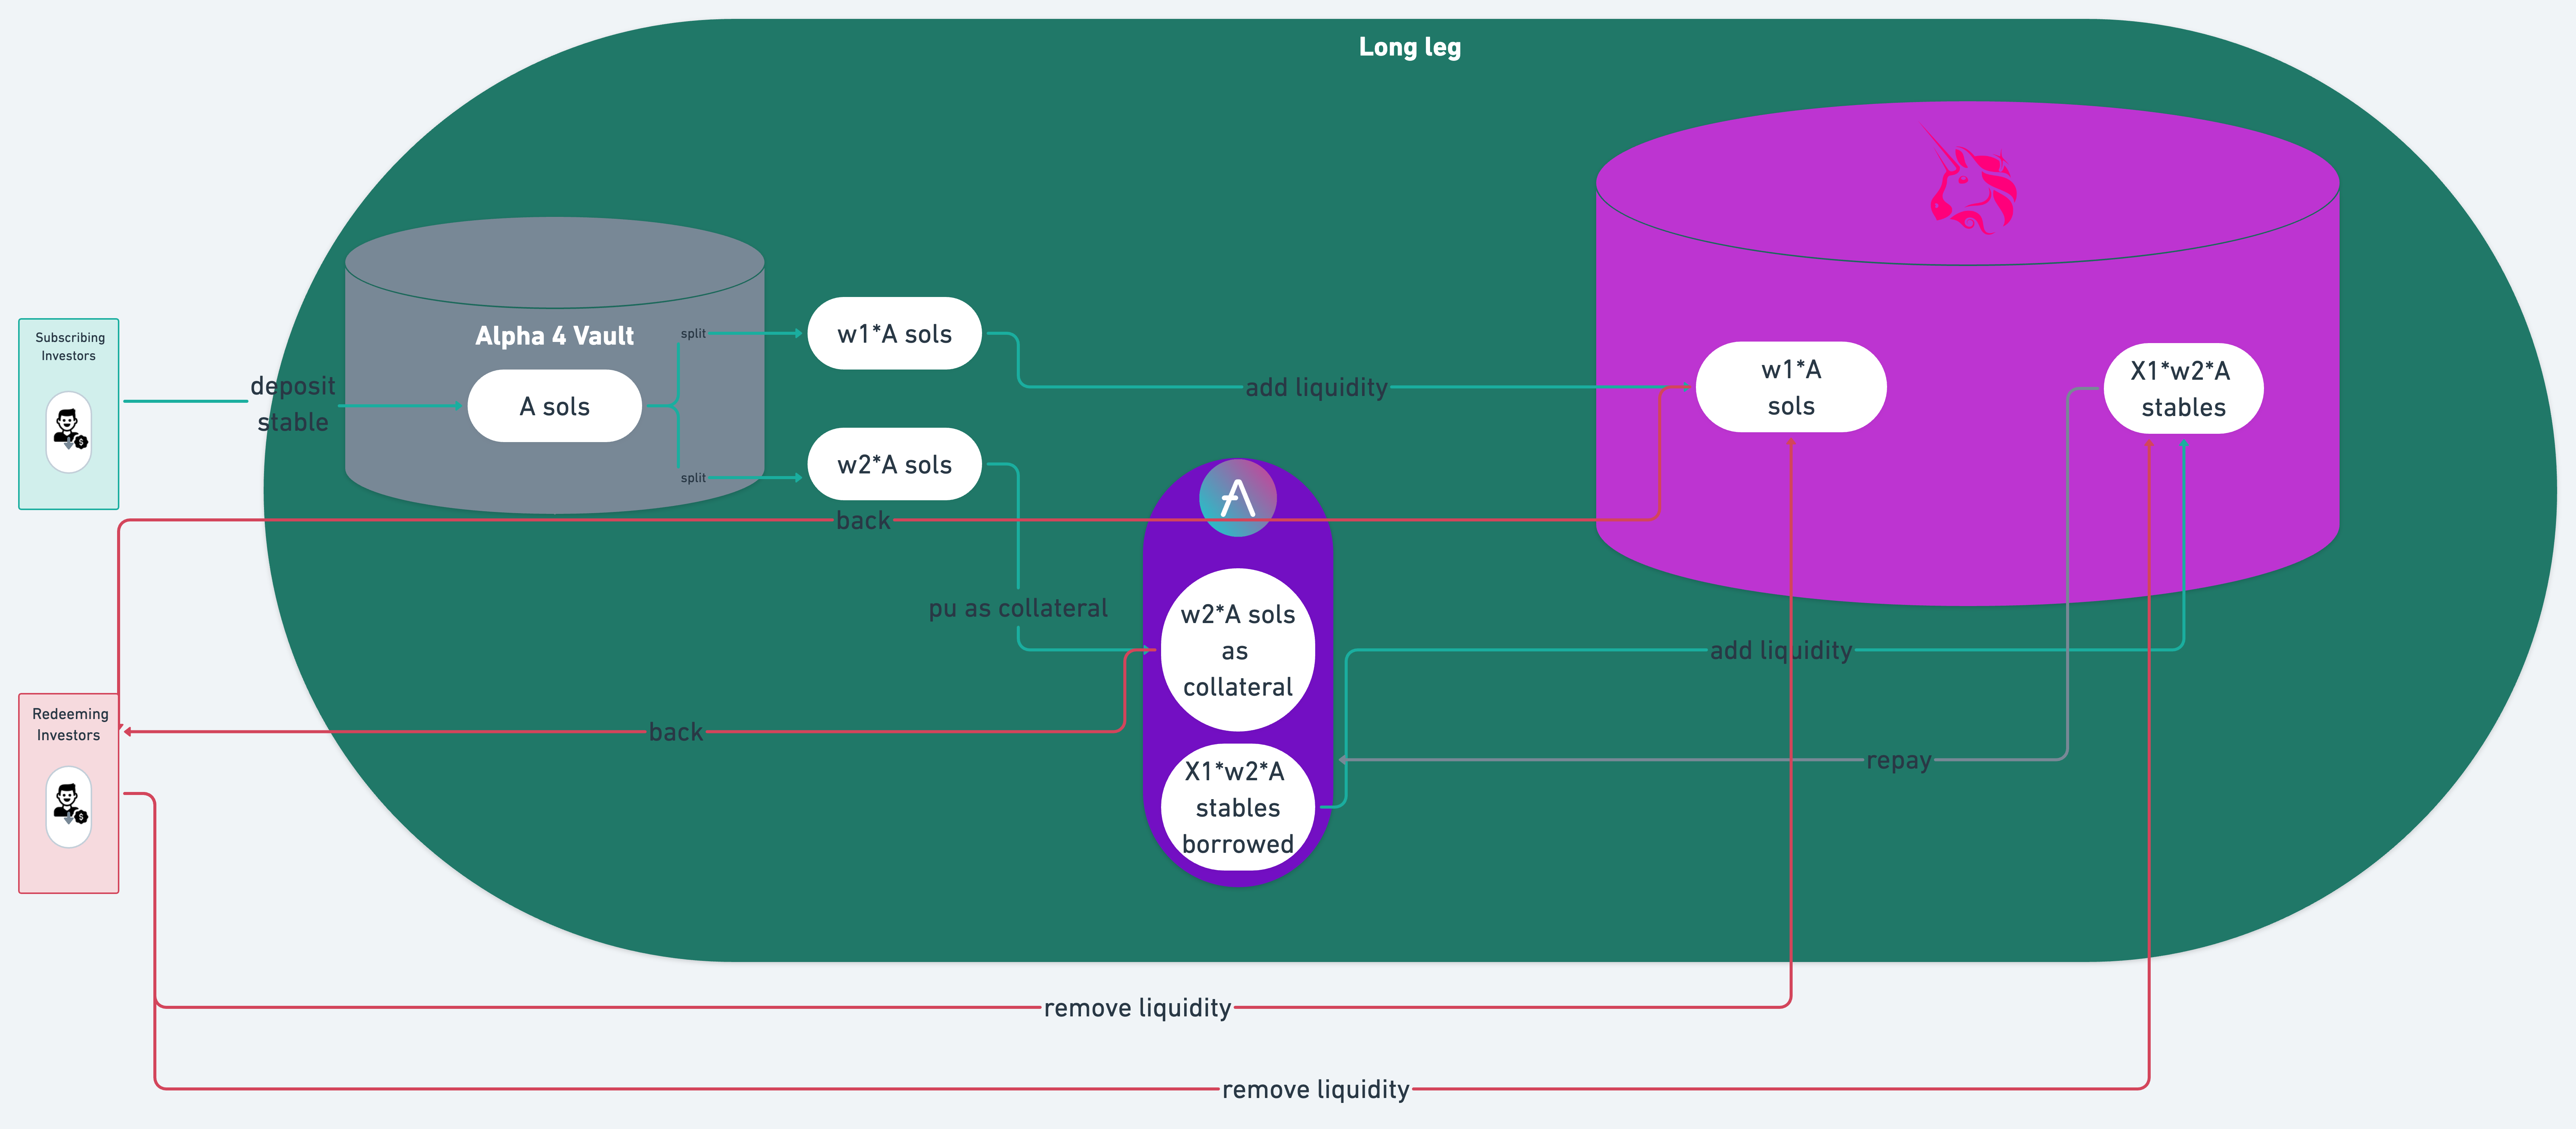
\includegraphics[scale=0.035]{Plots/long_leg.png}
    \caption{Long leg}
    \label{fig:conc_liquidity}
\end{figure}
The splitting quantities $\omega_1$ and $\omega_2$ must verify : 
\begin{equation}
\begin{array}{ll}
\omega_1 + \omega_2 = 1\\
\omega_1 * A = X_1*\omega_2 * A\\    
\end{array}
\end{equation}
, where $X_1$ is the collateral ratio : the amount of stable coins you can borrow against your Solana.\\
The solution is given by the splitting quantities :
\begin{equation}
\left\{
\begin{array}{ll}
\omega_1  = \frac{X_1}{1+X_1}\\
\omega_2  = \frac{1}{1+X_1}\\
\end{array}\right.
\end{equation}


\subsubsection{Short leg}
\begin{figure}[h!]
    \centering
    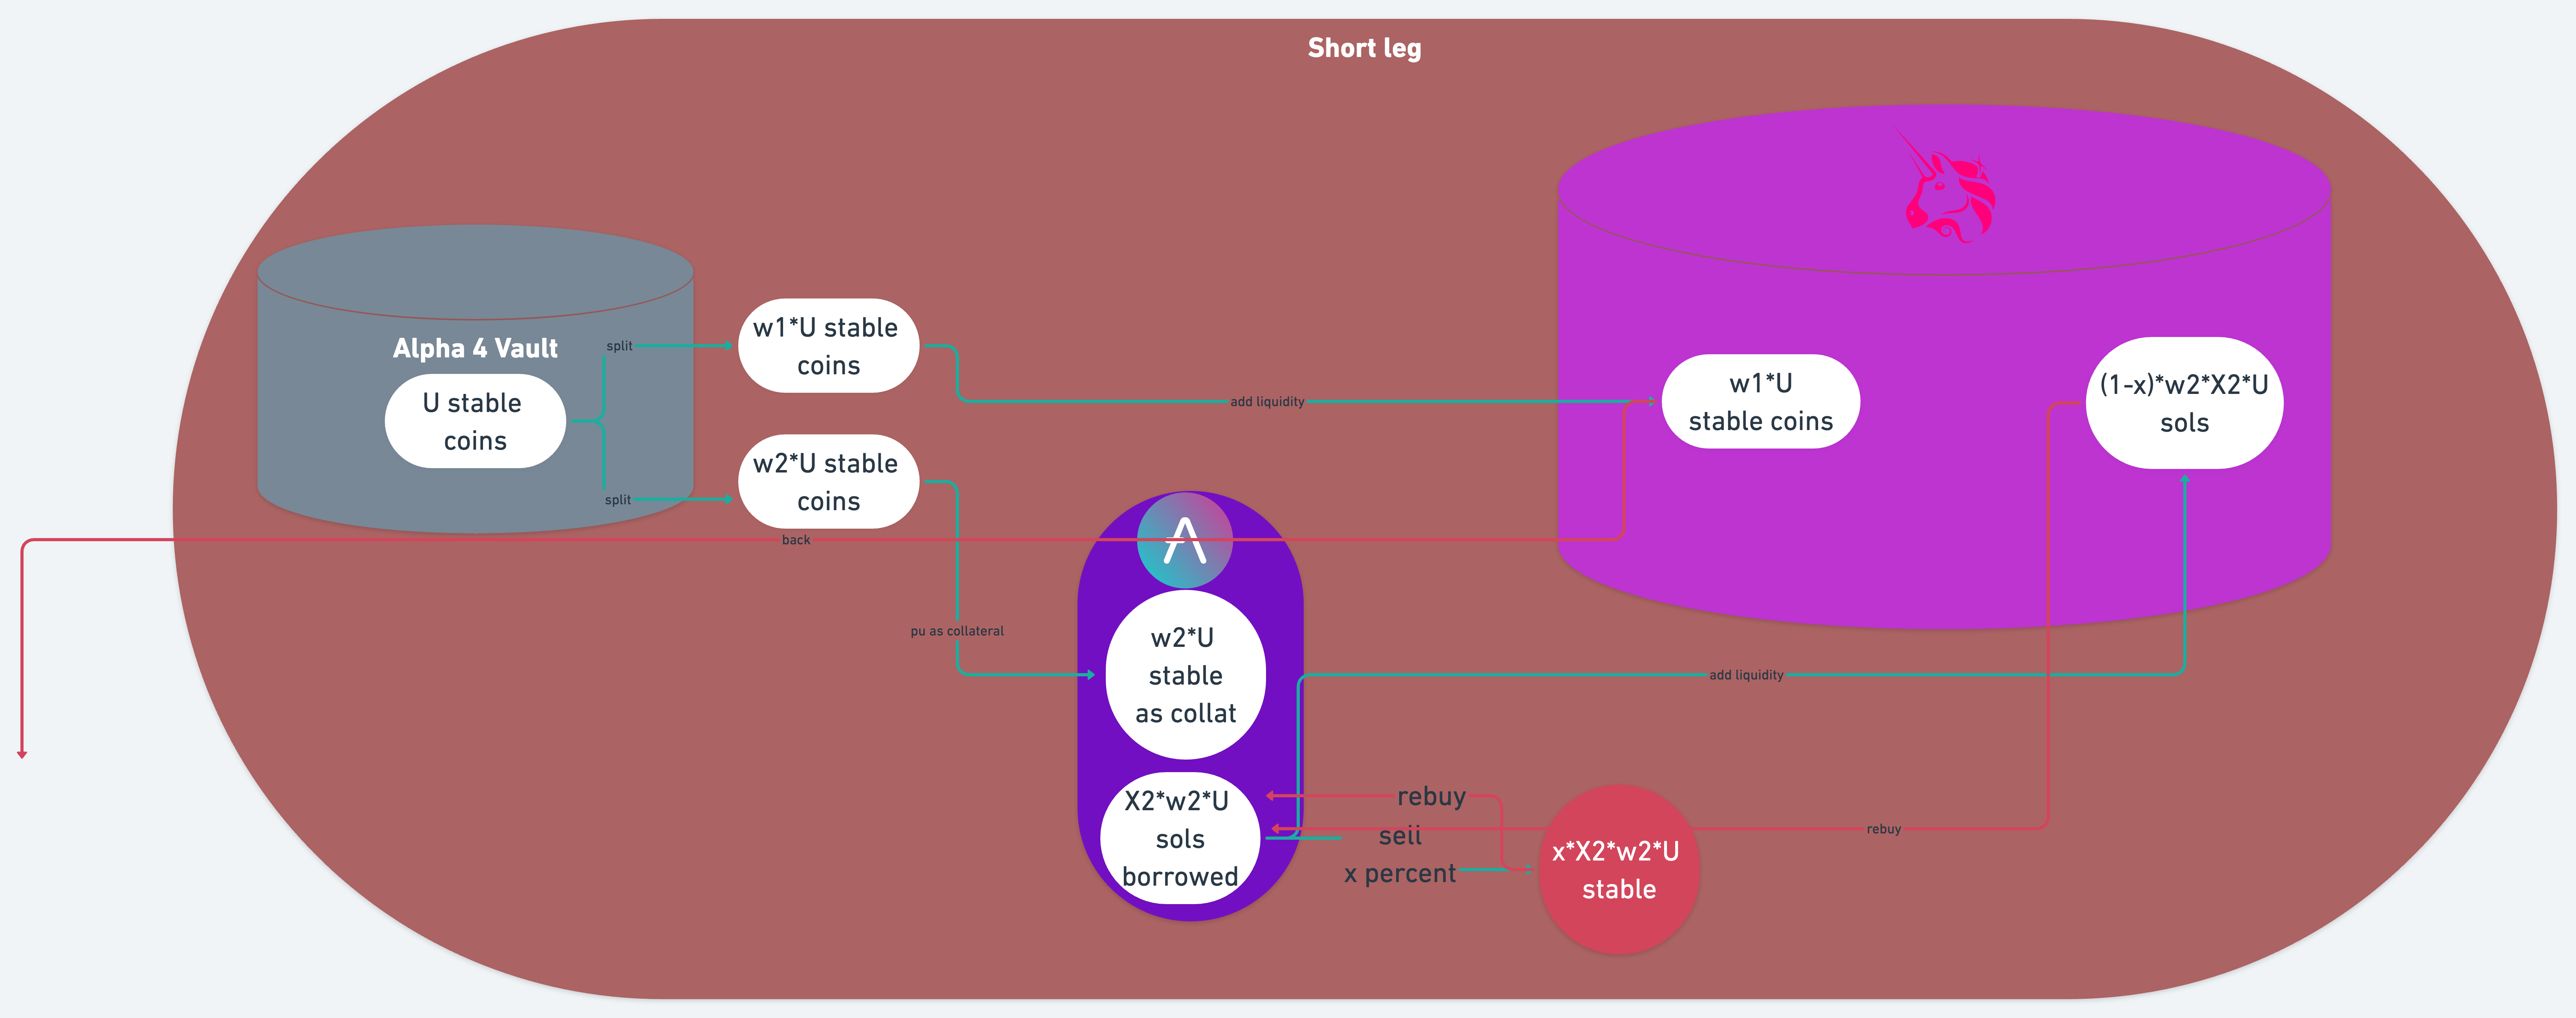
\includegraphics[scale=0.035]{Plots/short_leg.png}
    \caption{Short leg}
    \label{fig:conc_liquidity}
\end{figure}
The splitting quantities $\omega_1$ and $\omega_2$ must verify : 
\begin{equation}
\begin{array}{ll}
\omega_1 + \omega_2 = 1\\
\omega_1*U = (1-x)*\omega_2*X_2*U\\    
\end{array}
\end{equation}
, where $X_2$ is the collateral ratio : the amount of sols you can borrow against your stable coin and $x$ is the proportion of your borrowed Sols you use to short.\\
The solution is given by fixing the amount you have to short as a function of your liquidity position size $\omega_1$ ($x=f(\omega_1)$):
\begin{equation}
x = \frac{(1-\omega_1)*X2-\omega_1}{(1-\omega_1)*X2}
\end{equation}

\begin{figure}[h!]
    \centering
    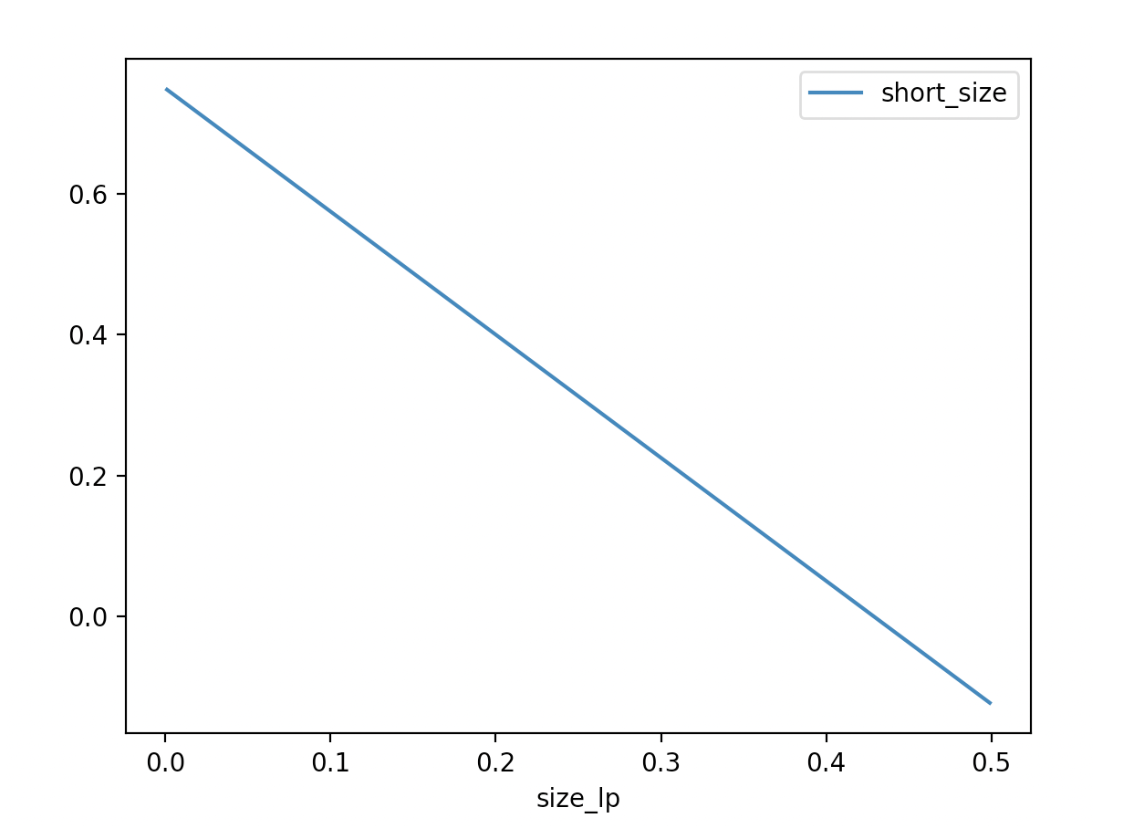
\includegraphics[scale=0.3]{Plots/short_size_as_lp_size.png}
    \caption{Long leg}
    \label{fig:conc_liquidity}
\end{figure}
We can see that the amount of short position we want to have will directly dictate the size of our LP position and therefore the fees we produce.\\
For a LP position of size 0, then $x=X_2$, meaning that we short the whole $\omega_2$ split from our asset.\\
For a LP of maximal size of $\omega_1 = \frac{1}{1+X_2}$ (roughly 55\%), then we have no room left to short : $x=0$.\\
For a LP size in between those bounds, it gives the following short position by noting : ${\text total-short-position} = S $\\
\begin{equation}
\begin{array}{ll}
S= x*(1-\omega_1)X2*U \\
S =  \left((1-\omega_1)*X2-\omega_1 \right)*U\\
\end{array}
\end{equation}\\
where $U$ is the amount of the stable coins at the beginning of the epoch.
The idea is to use that range of shorting size to adapt to our proprietary epoch market indicator by cumulating a long and a short leg simultaneously in an adaptating ratio.\\
By noting : ${\text total-long-position} = L $\ for a long leg.
\begin{equation}
L = A
\end{equation}\\where $A$ is the amount of risky coin at the beginning of the epoch.\\

So according to the risk level from our proprietary indicator for the next epoch, we can taylor the $\frac{short}{long}$ position ratio in a continuous way by allocating specific sizes of risky and numeraire asset:\\
\begin{equation}
\left\{
\begin{array}{lll}
\frac{A}{U} = \left((1-\omega_1)*X2-\omega_1 \right)\text{market neutral} \\
\frac{A}{U} > \left((1-\omega_1)*X2-\omega_1 \right) \text{long overall} \\
\frac{A}{U} < \left((1-\omega_1)*X2-\omega_1 \right)\text{short overall}  \\
\end{array}
\end{equation}


\subsubsection{Hedging with options instead of a short leg}
\subsubsubsection{Replicating the LP payoff}
We here investigate another way of mitigating our downside risk when assessing downside risky epoch.\\
We here propose to replicate the $LP$ value payoff at the end of an epoch by a basket of options whose maturity matches the end of the epoch.\\
We then optimize the options allocation to exactly fit the LP value payoff.\\

This can easily be done by an optimization algorithm minimizing the $L2$ norm between the LP payoff and the derivatives payoff.\\
We fetch from Derebit all options for a specific maturity. For each strike, we compute long/short versions of call/put payoffs:\\
\begin{equation}
\begin{array}{llll}
\text{Payoff Long Call} =  \max(0,P_f-K)\\
\text{Payoff Short Call} = -\max(0,P_f-K)\\
\text{Payoff Put Call} = \max(0,K-P_f)\\
\text{Payoff Long Call} = -\max(0,K-P_f)\\
\end{array}
\end{equation}
For a basket of weights $\theta=(\theta_i)$, we compute the final payoff:\\
\begin{equation}
Payoff(\theta, P_f) =\sum_{\theta_i in\theta}\theta_i*payoff_{\theta_i}(P_f)
\end{equation}
We then minimize the functional of the $L2$ distance between the two payoffs:
\begin{equation}
J(\theta) = \sum_{P_f in [0,+\infty[}(Payoff(\theta, P_f)-LP_{PnL}(P_f))^2
\end{equation}
This loss function can be optimized via Stochastic Gradient Descent. 
Each weight can be positive or negative. A positive value is a
long position in the options contract, while a negative value is a
short position.\\
We here under give an example of a replicated LP PnL at a one month expiry.
\begin{figure}[h!]
    \centering
    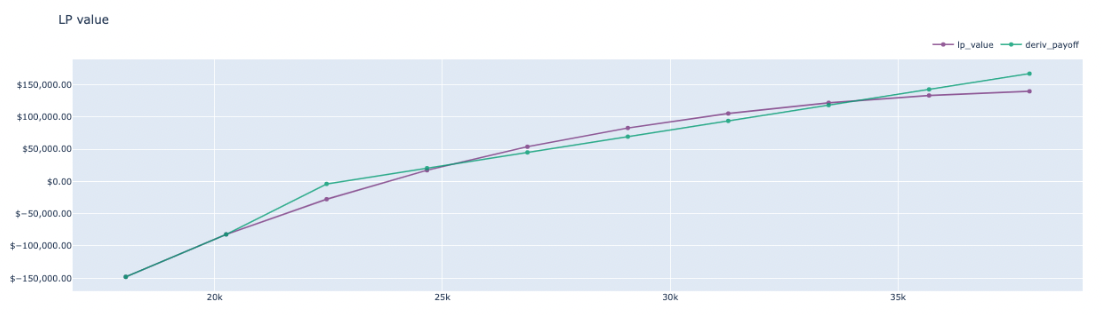
\includegraphics[scale=0.2]{Plots/option_hedging.png}
    \caption{Payoff replication using options}
    \label{fig:conc_liquidity}
\end{figure}
\subsubsubsection{Analyzing the hedging cost}
We can then analyse the total hedging cost by getting the options premium for Derebit and netting between the long and short premiums.
\begin{figure}[h!]
    \centering
    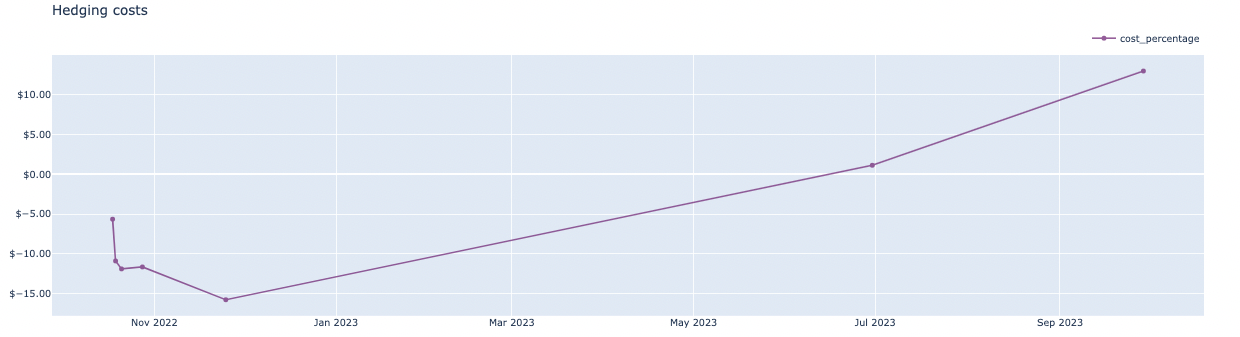
\includegraphics[scale=0.2]{Plots/hedging_costs.png}
    \caption{Hedging costs}
    \label{fig:conc_liquidity}
\end{figure}

%\section{Optimizing liquidity profile inside rangy market bounds}
%\subsection{Tick definition}
%Tick mathematical understanding is required to interpret both the values provided by the Uniswap v3 API and the data indexed %in the Uniswap v3.
%Uniswap v3 maps the continuous space of all possible prices to a discrete subset indexed by ticks.
%A tick has unique relation with price, defined by the tick base
%parameter, which is equal to 1.0001 in Uniswap (a one basis point deviation in price). The price corresponding to the i-th %tick is :
%\begin{equation}
%p(i) = {1.0001}^{i}
%\end{equation}
%However pools actually track ticks at every square root price that is an integer power of $\sqrt{1.0001}$. The tick i is %thus defined :
%\begin{equation}
%\sqrt{p(i)} = {\sqrt{1.0001}}^{i}
%\end{equation}
%\begin{equation}
%i_c = \left[\log_{\sqrt{1.0001}} \sqrt{P}\right]
%\end{equation}



\section{Conclusion}
https://medium.com/@RoboVault/delta-neutral-strategy-deep-dive-ae91d309b504
https://arxiv.org/abs/2208.03318
https://arxiv.org/pdf/2106.14404.pdf
https://uniswapv3.flipsidecrypto.com/
https://uniswaptimizer.com/
https://app.flipsidecrypto.com/velocity/queries/efed0457-5edc-46fa-ad7b-cffd01d5b93d
https://app.flipsidecrypto.com/velocity/queries/bb47119b-a9ad-4c59-ac4d-be8c880786e9
https://arxiv.org/pdf/2106.12033.pdf
https://medium.com/auditless/impermanent-loss-in-uniswap-v3-6c7161d3b445 

\bibliographystyle{IEEEtranN}
\bibliography{bib}
\nocite{*}
\end{document}

% to do
% Expliquer l'importance de la réduction de dimension dans ML
% Expliquer la diff CCA PCA pour ML